% Options for packages loaded elsewhere
\PassOptionsToPackage{unicode}{hyperref}
\PassOptionsToPackage{hyphens}{url}
%
\documentclass[
]{book}
\usepackage{lmodern}
\usepackage{amssymb,amsmath}
\usepackage{ifxetex,ifluatex}
\ifnum 0\ifxetex 1\fi\ifluatex 1\fi=0 % if pdftex
  \usepackage[T1]{fontenc}
  \usepackage[utf8]{inputenc}
  \usepackage{textcomp} % provide euro and other symbols
\else % if luatex or xetex
  \usepackage{unicode-math}
  \defaultfontfeatures{Scale=MatchLowercase}
  \defaultfontfeatures[\rmfamily]{Ligatures=TeX,Scale=1}
\fi
% Use upquote if available, for straight quotes in verbatim environments
\IfFileExists{upquote.sty}{\usepackage{upquote}}{}
\IfFileExists{microtype.sty}{% use microtype if available
  \usepackage[]{microtype}
  \UseMicrotypeSet[protrusion]{basicmath} % disable protrusion for tt fonts
}{}
\makeatletter
\@ifundefined{KOMAClassName}{% if non-KOMA class
  \IfFileExists{parskip.sty}{%
    \usepackage{parskip}
  }{% else
    \setlength{\parindent}{0pt}
    \setlength{\parskip}{6pt plus 2pt minus 1pt}}
}{% if KOMA class
  \KOMAoptions{parskip=half}}
\makeatother
\usepackage{xcolor}
\IfFileExists{xurl.sty}{\usepackage{xurl}}{} % add URL line breaks if available
\IfFileExists{bookmark.sty}{\usepackage{bookmark}}{\usepackage{hyperref}}
\hypersetup{
  pdftitle={Probability Theory and Statistics},
  pdfauthor={Malcolm Connolly},
  hidelinks,
  pdfcreator={LaTeX via pandoc}}
\urlstyle{same} % disable monospaced font for URLs
\usepackage{color}
\usepackage{fancyvrb}
\newcommand{\VerbBar}{|}
\newcommand{\VERB}{\Verb[commandchars=\\\{\}]}
\DefineVerbatimEnvironment{Highlighting}{Verbatim}{commandchars=\\\{\}}
% Add ',fontsize=\small' for more characters per line
\usepackage{framed}
\definecolor{shadecolor}{RGB}{248,248,248}
\newenvironment{Shaded}{\begin{snugshade}}{\end{snugshade}}
\newcommand{\AlertTok}[1]{\textcolor[rgb]{0.94,0.16,0.16}{#1}}
\newcommand{\AnnotationTok}[1]{\textcolor[rgb]{0.56,0.35,0.01}{\textbf{\textit{#1}}}}
\newcommand{\AttributeTok}[1]{\textcolor[rgb]{0.77,0.63,0.00}{#1}}
\newcommand{\BaseNTok}[1]{\textcolor[rgb]{0.00,0.00,0.81}{#1}}
\newcommand{\BuiltInTok}[1]{#1}
\newcommand{\CharTok}[1]{\textcolor[rgb]{0.31,0.60,0.02}{#1}}
\newcommand{\CommentTok}[1]{\textcolor[rgb]{0.56,0.35,0.01}{\textit{#1}}}
\newcommand{\CommentVarTok}[1]{\textcolor[rgb]{0.56,0.35,0.01}{\textbf{\textit{#1}}}}
\newcommand{\ConstantTok}[1]{\textcolor[rgb]{0.00,0.00,0.00}{#1}}
\newcommand{\ControlFlowTok}[1]{\textcolor[rgb]{0.13,0.29,0.53}{\textbf{#1}}}
\newcommand{\DataTypeTok}[1]{\textcolor[rgb]{0.13,0.29,0.53}{#1}}
\newcommand{\DecValTok}[1]{\textcolor[rgb]{0.00,0.00,0.81}{#1}}
\newcommand{\DocumentationTok}[1]{\textcolor[rgb]{0.56,0.35,0.01}{\textbf{\textit{#1}}}}
\newcommand{\ErrorTok}[1]{\textcolor[rgb]{0.64,0.00,0.00}{\textbf{#1}}}
\newcommand{\ExtensionTok}[1]{#1}
\newcommand{\FloatTok}[1]{\textcolor[rgb]{0.00,0.00,0.81}{#1}}
\newcommand{\FunctionTok}[1]{\textcolor[rgb]{0.00,0.00,0.00}{#1}}
\newcommand{\ImportTok}[1]{#1}
\newcommand{\InformationTok}[1]{\textcolor[rgb]{0.56,0.35,0.01}{\textbf{\textit{#1}}}}
\newcommand{\KeywordTok}[1]{\textcolor[rgb]{0.13,0.29,0.53}{\textbf{#1}}}
\newcommand{\NormalTok}[1]{#1}
\newcommand{\OperatorTok}[1]{\textcolor[rgb]{0.81,0.36,0.00}{\textbf{#1}}}
\newcommand{\OtherTok}[1]{\textcolor[rgb]{0.56,0.35,0.01}{#1}}
\newcommand{\PreprocessorTok}[1]{\textcolor[rgb]{0.56,0.35,0.01}{\textit{#1}}}
\newcommand{\RegionMarkerTok}[1]{#1}
\newcommand{\SpecialCharTok}[1]{\textcolor[rgb]{0.00,0.00,0.00}{#1}}
\newcommand{\SpecialStringTok}[1]{\textcolor[rgb]{0.31,0.60,0.02}{#1}}
\newcommand{\StringTok}[1]{\textcolor[rgb]{0.31,0.60,0.02}{#1}}
\newcommand{\VariableTok}[1]{\textcolor[rgb]{0.00,0.00,0.00}{#1}}
\newcommand{\VerbatimStringTok}[1]{\textcolor[rgb]{0.31,0.60,0.02}{#1}}
\newcommand{\WarningTok}[1]{\textcolor[rgb]{0.56,0.35,0.01}{\textbf{\textit{#1}}}}
\usepackage{longtable,booktabs}
% Correct order of tables after \paragraph or \subparagraph
\usepackage{etoolbox}
\makeatletter
\patchcmd\longtable{\par}{\if@noskipsec\mbox{}\fi\par}{}{}
\makeatother
% Allow footnotes in longtable head/foot
\IfFileExists{footnotehyper.sty}{\usepackage{footnotehyper}}{\usepackage{footnote}}
\makesavenoteenv{longtable}
\usepackage{graphicx,grffile}
\makeatletter
\def\maxwidth{\ifdim\Gin@nat@width>\linewidth\linewidth\else\Gin@nat@width\fi}
\def\maxheight{\ifdim\Gin@nat@height>\textheight\textheight\else\Gin@nat@height\fi}
\makeatother
% Scale images if necessary, so that they will not overflow the page
% margins by default, and it is still possible to overwrite the defaults
% using explicit options in \includegraphics[width, height, ...]{}
\setkeys{Gin}{width=\maxwidth,height=\maxheight,keepaspectratio}
% Set default figure placement to htbp
\makeatletter
\def\fps@figure{htbp}
\makeatother
\setlength{\emergencystretch}{3em} % prevent overfull lines
\providecommand{\tightlist}{%
  \setlength{\itemsep}{0pt}\setlength{\parskip}{0pt}}
\setcounter{secnumdepth}{5}
\usepackage{booktabs}
\usepackage{amsthm}
\usepackage{tikz}
\makeatletter
\def\thm@space@setup{%
  \thm@preskip=8pt plus 2pt minus 4pt
  \thm@postskip=\thm@preskip
}
\makeatother
\usepackage[]{natbib}
\bibliographystyle{apalike}

\title{Probability Theory and Statistics}
\author{Malcolm Connolly}
\date{Semester 2, 2023}

\usepackage{amsthm}
\newtheorem{theorem}{Theorem}[chapter]
\newtheorem{lemma}{Lemma}[chapter]
\newtheorem{corollary}{Corollary}[chapter]
\newtheorem{proposition}{Proposition}[chapter]
\newtheorem{conjecture}{Conjecture}[chapter]
\theoremstyle{definition}
\newtheorem{definition}{Definition}[chapter]
\theoremstyle{definition}
\newtheorem{example}{Example}[chapter]
\theoremstyle{definition}
\newtheorem{exercise}{Exercise}[chapter]
\theoremstyle{definition}
\newtheorem{hypothesis}{Hypothesis}[chapter]
\theoremstyle{remark}
\newtheorem*{remark}{Remark}
\newtheorem*{solution}{Solution}
\begin{document}
\maketitle

{
\setcounter{tocdepth}{1}
\tableofcontents
}
\hypertarget{intro}{%
\chapter{Introduction to Probability}\label{intro}}

Some things that happen are entirely predictable. For example, if one drops a ball from a height, we know it will hit the ground. Things that happen like this can be decribed as \emph{deterministic}. You may have heard people talk about things being written in the stars, or their fate, or destiny. The opinion that all things are pre-determined is called \emph{determinism}.

However, even if are a determinist, you will have to live with uncertainty. In our everyday lives we can think of examples where things happen that we cannot predict; a bus may be late, it may rain, or one might win the lottery. To one living with uncertainty, it is reasonable to quantify this uncertainty and act assuming outcomes are not pre-determined. If the outcome is not pre-determined then it is called \textbf{\emph{random}}.

The Mathematics of random phenomena is called Probability Theory. Most people have an intuitive idea of what is meant by probability or chance. Unfortunately Probability Theory is a subject in which there are endless examples of seemingly simple questions that turn out to be very complicated or have severely counter-intuitive answers.

\hypertarget{frequentist-perspective}{%
\section{Frequentist perspective}\label{frequentist-perspective}}

We need to start with some terminology.

\begin{definition}
\protect\hypertarget{def:experiment}{}\label{def:experiment}An \textbf{\emph{experiment}} is any procedure which happens at random with at least two different outcomes. For example rolling a die and observing the score is a statistical experiment. If the experiment is repeatable then each repetition is called a \textbf{\emph{run}}.
\end{definition}

By calculating the number of times an event occurs divided by the number of runs one can estimate the theoretical probability. The idea is that the relative cumulative frequency of outcomes will tend to the actual probability in the long run. This is perspective of probability is called \emph{Frequentist}, and is incredibly useful in practice.

gganim\_plot0100.png

We will recreate a plot like this in labs.

\begin{example}
\protect\hypertarget{exm:freq}{}\label{exm:freq}

Suppose we toss a \(10\) coins \(10\) times and the results are recorded in the table below, draw the graph of relative frequency.

\begin{longtable}[]{@{}lllllllllll@{}}
\toprule
Run & 1 & 2 & 3 & 4 & 5 & 6 & 7 & 8 & 9 & 10\tabularnewline
\midrule
\endhead
Outcome & 6H & 3H & 3H & 1H & 6H & 3H & 6H & 5H & 5H & 7H\tabularnewline
\bottomrule
\end{longtable}

The cumulative relative frequencies are calculated as the cumulative number of flips divided by the cumulative number of heads:

\begin{longtable}[]{@{}lllllllllll@{}}
\toprule
Cumulative flips \(n\) & 10 & 20 & 30 & 40 & 50 & 60 & 70 & 80 & 90 & 100\tabularnewline
\midrule
\endhead
Cumulative heads \(a_n\) & 6 & 9 & 12 & 13 & 19 & 22 & 28 & 33 & 38 & 45\tabularnewline
Relative Frequency & 0.6 & 0.45 & 0.4 & 0.325 & 0.38 & 0.367 & 0.4 & 0.413 & 0.422 & 0.45\tabularnewline
\bottomrule
\end{longtable}

\end{example}

In this course we will learn some R programming. R is a free open-source software language suitable for doing many probability and statistical calculations. The following R code will make a list of two outcomes Heads or Tails and create a sample of \(10\) random outcomes.

\begin{Shaded}
\begin{Highlighting}[]
\NormalTok{outcomes <-}\StringTok{ }\KeywordTok{c}\NormalTok{(}\StringTok{"Heads"}\NormalTok{,}\StringTok{"Tails"}\NormalTok{)}
\KeywordTok{sample}\NormalTok{(outcomes, }\DecValTok{10}\NormalTok{, }\DataTypeTok{replace=}\OtherTok{TRUE}\NormalTok{)}
\end{Highlighting}
\end{Shaded}

\begin{verbatim}
##  [1] "Tails" "Tails" "Heads" "Tails" "Heads" "Heads" "Tails" "Tails" "Tails"
## [10] "Tails"
\end{verbatim}

\begin{definition}
\protect\hypertarget{def:freq}{}\label{def:freq}If a statistical experiment has \(n\) runs, and the outcome \(A\) happens a cumulative number of times depending on \(n\) which we can call \(a_n\), then the \textbf{\emph{frequentist probability}} of the outcome \(A\), written \(P(A)\), is the limit:

\[P(A) = \lim_{n\to \infty} \frac{a_n}{n}\]
\end{definition}

So if it is possible to repeatedly run an experiment, frequentist methods are very useful for finding an approximation of the true theoretical probability.

Not all is so simple, consider the following questions. What is the probability that there is life on other planets? What is the probability that the Conservatives win the next general election?

These events are not like flipping a coin, and so it is not possible to find a frequentist interpretation for their probability.

\hypertarget{naive-probability}{%
\section{Naive probability}\label{naive-probability}}

We may not have the time or resources to do many thousands of runs. Therefore we also need to be able to evaluate the theoretical probability directly and exactly.

\begin{definition}
\protect\hypertarget{def:samplespace}{}\label{def:samplespace}The \textbf{\emph{sample space}} is a set whose elements are outcomes of an experiment. The sample space is denoted by the greek letter \(\Omega\).
\end{definition}

\begin{example}
\protect\hypertarget{exm:monthspace}{}\label{exm:monthspace}If we pick a person at random on the street and ask them the month of their birthday,
we can let
\[\Omega = \{\text{Jan}, \ \text{Feb}, \ \text{Mar},  \ \text{Apr}, \ \text{May}, \ \text{Jun}, \ \text{Jul}, \ \text{Aug}, \ \text{Sep}, \ \text{Oct}, \ \text{Nov}, \ \text{Dec} \}.\]
\end{example}

\begin{definition}
\protect\hypertarget{def:event}{}\label{def:event}An \textbf{\emph{event}} is a subset of the sample space \(\Omega\).
\end{definition}

\begin{example}
\protect\hypertarget{exm:landr}{}\label{exm:landr}As in example \ref{exm:monthspace}, let \(\text{L}\) be the \emph{event} that the month is a long month (i.e.~has 31 days). Then
\[\text{L} = \{\text{Jan}, \ \text{Mar}, \ \text{May},  \ \text{Jul}, \ \text{Aug},  \ \text{Oct}, \ \text{Dec} \}.\]

Let \(R\) be the \emph{event} that there is a letter \textbf{\emph{r}} in the name of the month when written fully. Here,

\[\text{R} = \{\text{Jan}, \ \text{Feb}, \ \text{Mar}, \ \text{Apr},  \ \text{Sep}, \ \text{Oct}, \ \text{Nov}, \  \text{Dec} \}\]
\end{example}

\begin{definition}
\protect\hypertarget{def:naiveprob}{}\label{def:naiveprob}Naively the the probability of an event \(A\) should be the number of elements of the set \(A\) divided by the size of the sample space \(\Omega\).That is,

\(\text{P} (A) = \frac{|A|}{|\Omega|}\).
\end{definition}

In our example \ref{exm:landr} above:

\[\text{P}(R) = \frac{|R|}{|\Omega|} = \frac{8}{12} = \frac{2}{3},\]

and,

\[\text{P}(L) = \frac{|L|}{|\Omega|} =\frac{7}{12}.\]

\begin{example}[Coin Tossing]
Toss a fair coin twice and record the possible outcomes. Let
\[A = \{\text{exactly one coin is Heads}\}\]
and
\[B = \{\text{neither coin is Heads}\}\]

The sample space here is \(\Omega = \{HH, HT, TH, HH\}\).

Events \(A\) and \(B\) correspond to:

\[A = \{HT, TH\}\]
and
\[B = \{ TT \}\]
Hence \(\text{P}(A) = \frac{2}{4} = \frac{1}{2}\), and \(\text{P}(B)=\frac{1}{4}\).
\end{example}

\begin{example}[Two dice]

Two dice are thrown, what is the probability that the total number of dots is:

\begin{enumerate}
\def\labelenumi{\alph{enumi})}
\tightlist
\item
  equal to \(7\)
\item
  equal to \(3\)
\item
  greater than \(5\)
\item
  an even number
\end{enumerate}

\emph{solution}

The sample space here is \(\Omega = \{ (n_1,n_2) : n_1 , n_2 \in \{1,2,3,4,5,6 \} \}\). However, not all sums are equally likely, which is best seen in a table.

\begin{longtable}[]{@{}ccccccc@{}}
\toprule
& 1 & 2 & 3 & 4 & 5 & 6\tabularnewline
\midrule
\endhead
1 & 2 & 3 & 4 & 5 & 6 & 7\tabularnewline
2 & 3 & 4 & 5 & 6 & 7 & 8\tabularnewline
3 & 4 & 5 & 6 & 7 & 8 & 9\tabularnewline
4 & 5 & 6 & 7 & 8 & 9 & 10\tabularnewline
5 & 6 & 7 & 8 & 9 & 10 & 11\tabularnewline
6 & 7 & 8 & 9 & 10 & 11 & 12\tabularnewline
\bottomrule
\end{longtable}

\begin{enumerate}
\def\labelenumi{\alph{enumi})}
\tightlist
\item
  \(\frac{6}{36}\)
\item
  \(\frac{2}{36}\)
\item
  \(\frac{26}{36}\)
\item
  \(\frac{18}{36}\)
\end{enumerate}

\end{example}

For infinite sets there is a problem with the naive definition \ref{def:naiveprob}. Consider the following:

\begin{example}
\protect\hypertarget{exm:randangle}{}\label{exm:randangle}Suppose a random unit vector is rotated about the origin anticlockwise, making an angle \(\theta\) with the positive \(x\)-axis. What is the probability that this angle is acute?

There are a continuum of infinitely many such angles. The naive definition says \(\frac{\infty}{\infty}\), which is absurd.

Intuitively, the answer \emph{should} be \(\frac{1}{4}\).
\end{example}

\hypertarget{complements-and-mutual-exclusivity}{%
\section{Complements and mutual exclusivity}\label{complements-and-mutual-exclusivity}}

In any case, as events are subsets of the sample space \(\Omega\) and follow the rules of set theory, and so it is important to know some set notation, definitions and results. Below is a recap of the important definitions.

\begin{definition}
\protect\hypertarget{def:union}{}\label{def:union}The \textbf{\emph{union}} of \(A\) and \(B\) is written:

\[A\cup B = \{ x \in \Omega :  x \in A \ \text{or} \ x\in B \}.\]
In Mathematics or is inclusive, which means we do not need to say ``or both'' as this is included in the union.
\end{definition}

\begin{definition}
\protect\hypertarget{def:intersection}{}\label{def:intersection}The \textbf{\emph{intersection}} of \(A\) and \(B\) is written:
\[A\cap B = \{ x \in \Omega:  x \in A \ \text{and} \ x\in B \}.\]
\end{definition}

\begin{definition}
\protect\hypertarget{def:mutex}{}\label{def:mutex}The empty set \(\varnothing\) is the set of no elements. As sets \(A\) and \(B\) are called disjoint if they have no elements in common, that is,

\(A \cap B = \varnothing.\)

In Probability Theory disjoint events are called \textbf{\emph{mutually exclusive}}.
\end{definition}

\begin{definition}
\protect\hypertarget{def:complement}{}\label{def:complement}The \textbf{\emph{complement}} of an event \(A\) is the event \(A^{c} = \{x \in \Omega : x\notin A\}.\)
Note \(A \cap A^{c} = \varnothing\). In words this means: any event is mutually exclusive with its complement.
\end{definition}

\begin{example}
Suppose the event is throwing a die. The event is that one throws an even number. The complement is that one throws an odd number.
\end{example}

\begin{example}
Suppose the event is that a random student has no siblings. The complement is not that they have one sibling. The complement is that they have \emph{at least} one sibling.
\end{example}

A theorem which we will not prove is De Morgan's laws

\begin{theorem}[DE MORGAN'S LAWS]
\protect\hypertarget{thm:demorgan}{}\label{thm:demorgan}The complement of a union is the intersection of the complements:
\[(A \cup B)^{c} = A^{c} \cap B^{c}\]

The complement of an intersection is the union of the complements:
\[(A \cap B)^{c} = A^{c} \cup B^{c}\]
\end{theorem}

In this way \(P\) is a `measure' function which maps the subsets of the sample space to the interval \(\left[0,1\right]\).

\begin{definition}
\protect\hypertarget{def:probability}{}\label{def:probability}

\textbf{\emph{Probability}} is a function whose input is a subset of the sample space \(A \subseteq \Omega\) and whose range is the interval \(\left[0,1\right]\), such that the following two axioms hold:

\begin{enumerate}
\def\labelenumi{(\roman{enumi})}
\item
  The probability of the whole set of possible events is unity. In the notation: \(\text{P}(\Omega ) =1\).
\item
  \emph{(additivity)} For any collection of disjoint events \(A_1 , A_2, A_3, \dots\) the probability of the union is the sum of the probabilities. In the notation this can be written as \[\text{P}(A_1 \cup A_2 \cup \dots ) = \text{P}(A_1) + \text{P}(A_2)+\dots .\]
\end{enumerate}

\end{definition}

The above definition \ref{def:probability} is due to the Russian Mathematician Kolmogorov. These axioms help make sense of the infinite case.

Using this definition we can prove the following important results.

\begin{proposition}[THE PROBABILITY OF A COMPLEMENT]
\protect\hypertarget{prp:sum}{}\label{prp:sum}For any event \(A\) we have:
\[\text{P}(A^{c}) = 1 - \text{P}(A).\]
\end{proposition}

\begin{proof}
Write \(\Omega = A \cup A^{c}\), which is a disjoint union. Then by additivity,
\[\text{P}(\Omega) = \text{P}(A) + \text{P}(A^{c}) \]
Now by axiom (i) the LHS is \(1\).
\end{proof}

\begin{theorem}[THE PROBABILITY OF A UNION]
\protect\hypertarget{thm:sum}{}\label{thm:sum}Given any two events \(A\) and \(B\) we have:

\[\text{P}(A\cup B) = \text{P}(A) + \text{P}(B) - \text{P}(A \cap B)\]
\end{theorem}

\begin{proof}
The idea is to write \(A\) as a disjoint union of the part that has intersection with \(B\), and that which does not: \(A=(A\cap B)\cup(A\cap B^{c})\). Hence,

\[\text{P}(A) = \text{P}(A\cap B) + \text{P}(A\cap B^{c})\]

If we split \(A\cup B\) in the same way, we obtain \((A\cup B)\cap B\) and \((A\cup B)\cap B^{c}\). The former is simply \(B\), and the latter is \(A \cap B^{c}\). Again by additivity,

\[\text{P}(A \cup B) = P(B) + P(A\cap B^{c}).\]
Eliminating \(P(A\cap B^{c})\) from the two equations above proves the rule.
\end{proof}

We will not be proving all Theorems in this course, neither will I ask you to recount a proof in an exam. You will however have to know how to use these results in applied problems.

\begin{example}[Multiple Choice]
Suppose a multiple choice test consists of three questions each of which has two options, the correct answer (C) or the wrong answer (W). What is the probability that a student who always randomly guesses the answers gets at least one correct?

\begin{align}
\text{P(at least one correct)} &= 1 - \text{P(all wrong)} \\
&= 1- \frac{1}{8}  \\
&=\frac{7}{8}
\end{align}
\end{example}

\begin{example}[Mode of travel]
The table shows the type of journey undertaken by a sample of commuters classified by where they live.

\begin{longtable}[]{@{}lccl@{}}
\toprule
& Town & Rural &\tabularnewline
\midrule
\endhead
Car & 40 & 30 & 70\tabularnewline
Bus & 25 & 5 & 30\tabularnewline
& 65 & 35 & 100\tabularnewline
\bottomrule
\end{longtable}

If an individual is selected at random from this group, find the probability that, they travel by car or live in the town

\emph{solution}

\(\text{P}(\text{Car}\cup \text{Town}) = \frac{25+40+30}{100}=0.95\)

\(\text{P}(\text{Car})+ \text{P}(\text{Town})-\text{P}(\text{Car}\cap \text{Town})= \frac{65}{100}+\frac{70}{100}-\frac{40}{100} =0.95\)
\end{example}

\begin{example}
In a particular city \(60\%\) of people watch the news in the morning, \(50\%\) of people watch the news in the evening and \(30\%\) watch both. What is the probability that an individual selected at random watches either the morning news or the evening news.

\emph{solution}

\(\text{P}(M\cup E) = 0.6 + 0.5 - 0.3 = 0.8\)
\end{example}

\hypertarget{outcomes-and-counting}{%
\section{Outcomes and counting}\label{outcomes-and-counting}}

One might imagine that the finite situation is then very simple, and even then we have seen this is not the full picture. One simply counts how many ways an event can happen out of the total number of configurations. This can actually be quite complicated. We will learn some formulae to enable us to count them.

\hypertarget{factorials}{%
\subsection{Factorials}\label{factorials}}

\begin{example}[Three people in a line]
\protect\hypertarget{exm:three}{}\label{exm:three}In how many ways can three people \(A\), \(B\) and \(C\) stand in a line?

\emph{solution}

\(ABC, ACB, BAC, BCA, CAB,CBA\) there are \(6\).
\end{example}

\begin{definition}
For any non-negative integer, \(n\) say, we define the factorial of \(n\), written \(n!\) to be equal to the product of \(n\) and all the numbers less than \(n\) down to \(1\). That is,

\[n! = n \times (n-1) \times (n-2) \times \dots 3 \times 2 \times 1\]
\end{definition}

\begin{definition}[Multiplication Rule]
If there are \(n\) ways for some operation to happen, and \(m\) ways for something else to happen, then the total number of ways for the sequence to occur is \(n \times m\).
\end{definition}

\begin{example}
MMU assigns each student an \(8\) digit ID number. How many possible ID numbers are there?

\emph{solution}
The first digit is not zero, there are \(9\) digits from which to choose.
All the other digits have \(10\) choices \(0,1,2,3,4,5,6,7,8,9\).

Total = \(9 \times 10^7\).
\end{example}

\begin{example}[objects in a line]
The number of ways of arranging \(n\) distinct objects in a line is \(n!\).
This is because there are \(n\) choices for the first number in line, then one fewer choice \((n-1)\) for the second, and so on, until the last one in the line there is only one choice remaining.
\end{example}

\begin{definition}[rule of division]
The number of ways of arranging \(n\) objects in a line where \(p\) are the same is \(\frac{n!}{p!}\).
\end{definition}

\begin{example}
\leavevmode

\begin{enumerate}
\def\labelenumi{\alph{enumi})}
\item
  Suppose you have the letters \(A,A,A,B\) - how many `words' can be made?
\item
  Suppose you have the letters \(A,A,A,B,B\) - how many `words' can be made?
\end{enumerate}

\emph{solution}
a)
AAAB, AABA, ABAA, BAAA

There are 4. How to find this number without having to write them down?

You might think \(4!\) but this is thinking each A is different, and so overcounts the same word. By what factor does it overcount? Take one of the words such as ABAA and number each A, one finds rearrangements of 1,2,3:

\(A_1BA_2A_3, A_1BA_3A_2, A_2BA_1A_3, A_2BA_3A_1, A_3BA_1A_2, A_3BA_2A_1.\)

The upshot is that you need to divide by the factorial of number of letters that are the same, here \(\frac{4!}{3!} =4\).

\begin{enumerate}
\def\labelenumi{\alph{enumi})}
\setcounter{enumi}{1}
\tightlist
\item
  Here there are \(3\) of the same letter \(A\), and \(2\) of the same letter \(B\). The correct number is
\end{enumerate}

\[\frac{5!}{3!\times2!} = 10\]

The words are AAABB, AABBA, ABBAA, BBAAA, BABAA, ABABA, AABAB, BAABA, ABAAB, BAAAB. (Here I can systematically list them by considering the number of A's between the B's).

\end{example}

\begin{definition}[rule of sum]
Given two disjoint events \(A\) and \(B\), then the size of the union is the sum of the sizes of \(A\) and \(B\). That is,

\[|A\cup B|=|A|+|B|\]
\end{definition}

\begin{example}
How many possible MMU IDs start with a \(1\) or a \(3\)?

\emph{solution}

The IDs are all of the form 1******* or 3*******. There is only 1 choice for the first digit and \(10^7\) choices for the next digits in either case.

The total number starting with a \(1\times 10^7 + 1\times 10^7 = 2\times 10^7.\)
\end{example}

\hypertarget{permutations}{%
\subsection{Permutations}\label{permutations}}

\begin{example}
Consider the number of ways of placing three of the letters \(A,B,C,D,E,F G\) in three empty spaces. The first space can be filled in \(7\) ways, the second in \(6\) ways and the last in \(5\) ways.

In total this is \(7\times 6\times 5 = 120\)

This number can be written as
\[\frac{7\times 6 \times 5\times 4\times 3\times 2\times 1}{4\times 3 \times 2\times 1}=\frac{7!}{(7-3)!}\]
\end{example}

\begin{definition}[Permutations]
The number of ways of choosing \(k\) distinct items from \(n\) when the order is relevant is
\[^n\text{P}_k = \frac{n!}{(n-k)!}\]
Any way of choosing \(k\) distinct items from \(n\) when order matters is called a \textbf{\emph{permutation}}.
\end{definition}

\begin{example}
My PIN has \(4\) different digits. How many different such PINs are there?

\emph{solution}

Order matters here - the guess 1234 is different from 4321, for example.

\[^{10}\text{P}_4 = \frac{10!}{(10-4)!} = \frac{10\times 9 \times \dots 2 \times 1 }{6!} =10\times 9 \times 8 \times 7 =5040\]
The expression \(10\times 9 \times 8 \times 7\) can be interpreted as saying there are \(10\) choices for the first digit, \(9\) or the second, and so on.
\end{example}

\begin{example}[The Birthday Problem]
\protect\hypertarget{exm:birthday}{}\label{exm:birthday}Suppose there are \(k\) people in a room. What is the probability that at least one has the same birthday as someone else in the room?

\emph{solution}

\[\text{P}(\text{at least one birthday the same}) = 1 - \text{P}(\text{all birthdays different})\]

The first person could be born on any day there are \(365\) such days, the second person has to have a different birthday so that is \(364\) and so on down to the \(k^{th}\) person.

\(\text{P}(\text{all birthdays different}) = \frac{^{365}\text{P}_k}{365^k}\)

This can be evaluated on a computer for different values of \(k\).

When \(k=23\) one finds \(\text{P}(\text{all birthdays different}) = 0.493\).

This implies that \(\text{P}(\text{at least one birthday the same}) = 1- 0.493 > 0.5\).

There is a greater than evens chance of two people having the same birthday in a room of \(23\) people.
\end{example}

\hypertarget{combinations}{%
\subsection{Combinations}\label{combinations}}

\begin{definition}[Combinations]
\protect\hypertarget{def:comb}{}\label{def:comb}The number of ways of choosing \(k\) distinct items from \(n\) when the order is not relevant is:

\[{}^nC_k = \frac{n!}{(n-k)!k!}\]
A way of choosing \(k\) distinct items from \(n\) when order does not matter is called a \textbf{\emph{combination}}.
\end{definition}

\begin{example}
In how many ways can \(4\) cards be dealt from an ordinary pack of \(52\) playing cards?

\emph{solution}

Suppose one such hand is the Ace of spades, the king of clubs, the three of hearts and the Jack of diamonds. It does not matter which card you were given first, as the hand is all that matters to play.

Here `order does not matter'.

The number of hands is \({}^{52}C_{4}=270725\).
\end{example}

\begin{example}[The National Lottery]
In the main National Lottery draw, six numbers are chosen from \(49\).

\begin{enumerate}
\def\labelenumi{\alph{enumi})}
\item
  What is the probability of winning the jackpot on the lottery (i.e.~all \(6\) match)?
\item
  What is the probability that three of the winning numbers come up on a lottery ticket?
\end{enumerate}

\emph{solutions}

\begin{enumerate}
\def\labelenumi{\alph{enumi})}
\tightlist
\item
  Total number of outcomes \({}^{49}C_{6} = 13983816\).
\end{enumerate}

The probability is \(\frac{1}{^{49}C_{6}}\), which is about \(1\) in \(14\) million.

\begin{enumerate}
\def\labelenumi{\alph{enumi})}
\setcounter{enumi}{1}
\tightlist
\item
  The three winning numbers can be any three of the six winning numbers with \(^6C_3\) combinations. The other numbers on the ticket can be any three from the \(43\) losing numbers that week. The number of ways of choosing these is \(^{43}C_3\).
\end{enumerate}

Therefore the probability of three winning numbers is
\[\text{P}(\text{three winning numbers}) = \frac{^{43}C_3 \times ^6C_3}{^{49}C_6} = 0.0177\]
This is approximately \(1\) in \(56\).
\end{example}

\hypertarget{exercises-week-1}{%
\section{Exercises Week 1}\label{exercises-week-1}}

\hypertarget{tutorial-exercises}{%
\subsection{Tutorial exercises}\label{tutorial-exercises}}

\begin{exercise}
A letter is chosen at random from the word STATISTICS.
a) What is the probability that it is a vowel?
b) What is the complement of the event in a)?
\end{exercise}

\begin{exercise}
Suppose you are eating in a restaurant with two friends. You agree to pay the bill as follows. Each person tosses a coin. The person who gets a result different from the other two will pay all the bill. If all three tosses are the same, the bill will be shared equally. Find the probability that:

\begin{enumerate}
\def\labelenumi{\alph{enumi})}
\tightlist
\item
  Only you will pay the bill
\item
  All three will share the bill
\end{enumerate}

Do you think this is a \emph{fair} way to split the bill?
\end{exercise}

\begin{exercise}
\protect\hypertarget{exr:invest}{}\label{exr:invest}

An investment can either; increase in value (I), break even (B) or make a loss (L). Suppose each outcome is equally likely. If two separate investments are made,

\begin{enumerate}
\def\labelenumi{\alph{enumi})}
\item
  List the sample space by drawing a tree diagram.
\item
  Find the probability that:
\end{enumerate}

\begin{enumerate}
\def\labelenumi{(\roman{enumi})}
\tightlist
\item
  both investments increase in value.
\item
  both investments make a loss.
\item
  At least one of the investments increases in value.
\end{enumerate}

\begin{enumerate}
\def\labelenumi{\alph{enumi})}
\setcounter{enumi}{2}
\tightlist
\item
  Suppose both investments were in the same type of company. How might this model be unrealistic, and how could you improve it?
\item
  How big would the sample space be if three separate investments were made?
\end{enumerate}

\end{exercise}

\begin{exercise}

A set of cards consists of the standard suits \(\clubsuit\), \(\spadesuit\), \(\diamondsuit\), \(\heartsuit\), with \(13\) cards in each suit.
a) Suppose one card is drawn at random. Find the probability that it is a:
(i) Ace of Hearts, \(A\heartsuit\)
(ii) The King of Spades \(K\spadesuit\).
(iii) Any picture card.

\begin{enumerate}
\def\labelenumi{\alph{enumi})}
\setcounter{enumi}{1}
\tightlist
\item
  Suppose two cards are drawn at random, but with the first being replaced and the deck shuffled before the second is drawn ( this is called sampling with replacement). Find the probability that:
\end{enumerate}

\begin{enumerate}
\def\labelenumi{(\roman{enumi})}
\tightlist
\item
  Both cards are the King of Hearts, \(K\heartsuit\).
\item
  Both cards are Aces.
\end{enumerate}

\end{exercise}

\begin{exercise}
Fifty male and fifty female students were asked whether they agreed with the statement ``Statistics are often misleading''. Seventy students, thirty of whom were male, agreed.
a) Summarise this information in a two-way table.
b) If a student is selected at random, find the probability that they:
(i) Agree
(ii) Are female
(iii) Are male
(iv) Are male and agree
(v) Are female or agree
\end{exercise}

\begin{exercise}
Interviews with \(120\) working people revealed that \(76\) were stressed, \(20\) were managers and \(14\) were both managers and stressed.
a) Summarise this information in a two-way table.
b) Assuming an individual is drawn at random, find the probability thatthey are
(i) Stressed
(ii) A shopfloor worker
(iii) A manager who is stressed
(iv) A shopfloor worker or is not stressed.
\end{exercise}

\begin{exercise}
Evaluate a) \(^5\text{P}_3\), b) \(^7\text{P}_4\), c) \(^6\text{P}_4\).
\end{exercise}

\begin{exercise}
For what value of \(n\) is the following equality true?
\[ ^{n+1}\text{P}_3 = ^n\text{P}_4 \]
\end{exercise}

\begin{exercise}
Three different Mathematics books and \(5\) different statistics books are to be arranged on a shelf. In how many ways can the books be arranged if,
a) The books in each subject must stand together
b) Only the statistics books must stand together
\end{exercise}

\begin{exercise}
Four different Mathematics books, \(5\) different statistics books and \(3\) different computing books are to be arranged on a shelf. In how many ways can the books be arranged if,
a) The books in each subject must stand together
b) Only the statistics books must stand together
\end{exercise}

\begin{exercise}
Evaluate a) \(^7\text{C}_6\), b) \(^5\text{C}_3\), c) \(^9\text{C}_5\), \(^9\text{C}_4\).
\end{exercise}

\begin{exercise}
How many different committees can be formed from \(8\) men and \(6\) women if the committee consists of:
a) \(1\) man and \(4\) women
b) \(5\) men and \(3\) women
c) \(4\) men and \(4\) women
d) An equal number of men and women.
\end{exercise}

\begin{exercise}
A council consists of \(10\) members, \(6\) from Party X and \(4\) from Party \(Y\).
a) In how many ways can a committee of \(4\) be formed?
b) In how many ways can a committee of \(4\) be formed so that:
i) Party X has the majority
ii) Party Y has the majority
iii) Neither party has the majority
\end{exercise}

\begin{exercise}
Ten equally qualified assistant managersare lined up for promotion. Seven are men and three are women. If the company promotes four of the ten at random, what is the probability that exactly two of the four chosen are women?
\end{exercise}

\begin{exercise}
Suppose a library bookshelf contains an equal number, \(n\) each say, of Mathematics books and Physics books. If the bookshelf is emptied and the books placed back randomly, what is the probability that the books for each subject are separated?
\end{exercise}

\begin{exercise}
Here are some miscellaneous questions on permutations and combinations:
a) From a group of \(20\) employees, \(4\) are chosen for promotion. In how many ways can they be chosen?
b) From a group of \(20\) employees, \(4\) are shosen for promotion, but each to a different role. In how many ways can they be chosen?
c) A product code consists of \(4\) letters followed by \(3\) digits. How many codes are possible if repetitions are not allowed?
d) A \(7\)-card hand is dealt from a normal pack of \(52\) cards. How many hands will contain \(4\) clubs and \(3\) hearts?
e) How many ways can merit awards be allocated to a group of \(15\) students if there is one first prize, one second prize and \(4\) identical third prizes?
f) Four students are to be chosen from a group of \(10\). If exactly \textbf{\emph{one}} of the first three students must be chosen, how many ways are there of choosing the four students?
\end{exercise}

\begin{exercise}
In the game of poker, five cards from a standard deck of \(52\) cards are dealt in a hand. Find the probability that a hand contains,
a) A royal flush (ace, king, queen, jack and \(10\) of the same suit)
b) Four of a kind (e.g.~all four \(5\)s)
c) Two pairs
d) A full house (i.e.~three of one kind and two of another)
e) One pair
\end{exercise}

\begin{exercise}
If \(\text{P(A)}=0.6\) and \(\text{P(B)}=0.5\), can A and B be mutually exclusive?
\end{exercise}

\begin{exercise}

The medical records of \(100\) male diabetic patients reported to a clinic their family history of diabetes (Yes or No), together with their symptoms as either mild or severe. This provided the following classification.

\begin{longtable}[]{@{}crr@{}}
\toprule
Age & Mild and Yes & Mild and No\tabularnewline
\midrule
\endhead
under 40 & 15 & 10\tabularnewline
40 or over & 15 & 20\tabularnewline
\bottomrule
\end{longtable}

\begin{longtable}[]{@{}crr@{}}
\toprule
Age & Severe and Yes & Severe and No\tabularnewline
\midrule
\endhead
under 40 & 8 & 2\tabularnewline
40 or over & 20 & 10\tabularnewline
\bottomrule
\end{longtable}

Suppose a patient is chosen at random from this clinic and the events A, B and C are defines as follows:

A : He has a severe disease

B : He is under \(40\)

C : His parents are diabetic

\begin{enumerate}
\def\labelenumi{\alph{enumi})}
\item
  Find the probabilities P(A), P(B), P(A\(\cap\)B), P(B\(\cap\)C), P(A\(\cap\)B\(\cap\)C).
\item
  Describe the following events in words and calculate them: A\(^c\cap\)B\(^c\), A\(^c\cup\)C\(^c\), A\(^c\cap\)B\(^c\cap\)C\(^c\).
\end{enumerate}

\end{exercise}

\hypertarget{exercises-for-feedback}{%
\subsection{Exercises for feedback}\label{exercises-for-feedback}}

\begin{enumerate}
\def\labelenumi{\arabic{enumi}.}
\tightlist
\item
  I cannot remember a phone number. It contains the following digits and is something like \(132 \ 747 \ 6965\).
\end{enumerate}

\begin{enumerate}
\def\labelenumi{\alph{enumi})}
\item
  What is the probability that the first number is even?
\item
  How many ways can the numbers above be rearranged?
\item
  In how many ways can the number be rearranged to start and end with an odd number?
\end{enumerate}

Suppose I am certain of the numbers in each of the blocks \(132\),\(747\) and \(6965\), but not am not sure of the order within each block.

\begin{enumerate}
\def\labelenumi{\alph{enumi})}
\setcounter{enumi}{2}
\item
  How many ways can the numbers be rearranged such that the numbers within each block are the same?
\item
  What is the probability that I wrote down the correct number originally?
\end{enumerate}

\begin{enumerate}
\def\labelenumi{\arabic{enumi}.}
\setcounter{enumi}{1}
\tightlist
\item
  In a lottery, \(6\) numbers are drawn from the numbers \(1\) to \(49\). Calculate the following probabilities.
\end{enumerate}

\begin{enumerate}
\def\labelenumi{\alph{enumi})}
\item
  The numbers \(1\), \(2\), \(3\), \(4\), \(5\), \(6\) are all drawn.
\item
  The numbers \(4\), \(23\), \(24\), \(35\), \(40\), \(45\) are all drawn.
\item
  \(44\) is one of the numbers drawn.
\end{enumerate}

\begin{enumerate}
\def\labelenumi{\arabic{enumi}.}
\setcounter{enumi}{2}
\tightlist
\item
  Three dice are rolled. The sum of the numbers on the dice is the score.
\end{enumerate}

\begin{enumerate}
\def\labelenumi{\alph{enumi})}
\item
  Describe the sample space.
\item
  How many ways could the score equal \(5\)?
\item
  What is the most likely score?
\end{enumerate}

\begin{enumerate}
\def\labelenumi{\arabic{enumi}.}
\setcounter{enumi}{3}
\tightlist
\item
  Suppose we have a finite set \(S\) of size \(n\).
  (Hint: this question is general, but you could check your answers with concrete example S = \{ a,b,c,d \})
\end{enumerate}

\begin{enumerate}
\def\labelenumi{\alph{enumi})}
\item
  How many subsets are there of \(S\)?
\item
  How many subsets of S are there of size \(1\)?
\item
  How many subsets of S are there of size \(k\), where \(1\leq k\leq n\)
\item
  Using a) and c), describe in words why the following equality holds.
\end{enumerate}

\[2^n = \sum_{k=0}^n {^n}C_k\]

\begin{enumerate}
\def\labelenumi{\arabic{enumi}.}
\setcounter{enumi}{4}
\tightlist
\item
  Five office workers write their names on a piece of paper, fold the paper and put them in a hat. The names are mixed up and each person then selects a piece of paper from the hat. After everyone has selected a piece of paper from the hat, the staff look at the names drawn. What is the probability that no member of staff selected their own name?
\end{enumerate}

\hypertarget{cond}{%
\chapter{Conditional Probability}\label{cond}}

In this chapter we will learn about conditional probability. This is the probability of an event, in the context of another event having happened or potentially happening.

\hypertarget{independence}{%
\section{Independence}\label{independence}}

Independence is a very important concept in Statistics, but one that is sometimes misused when it is assumed without justification. The basic idea is as follows:

\begin{definition}[Independence]
Two events \(\text{A}\) and \(\text{B}\) are \textbf{\emph{independent}} exactly when
\[\text{P}(\text{A}\cap\text{B}) = \text{P}(\text{A})\times \text{P}(\text{B}).\]
In words this means the probability that both \(\text{A}\) and \(\text{B}\) happen is the product of the individual probabilities of \(\text{A}\) and \(\text{B}\) respectively.
\end{definition}

\begin{example}

Some events that can be modelled as \textbf{\emph{independent}} include:
- Outcomes on successive tosses of a coin or die. What happened on the previous throw does not affect what happens on subsequent throws.

\begin{itemize}
\tightlist
\item
  The sex of babies. The sex of each baby is determined at random, notwithstanding the sexes of previous babies.
\end{itemize}

\end{example}

\begin{example}
Suppose a power plant has two safety systems, a primary system which works with probability \(0.999\), and a backup system which works with probability \(0.89\) Assuming that the two systems operate independently, what is the reliability or safety of the power plant.

\emph{solution}

We can work out \(\text{P}(\text{plant safe})\) using the complement:

\[\text{P}(\text{plant safe}) = 1-\text{P}(\text{plant fails}).\]

Let \(F\) be the event that the plant fails, \(F_1\) the event that the first system fails, and \(F_2\) the backup fails.

Then \(F = F_1 \cap F_2\).

\begin{align}
\text{P}(F) &= \text{P}(F_1 \cap F_2) \\
&= \text{P}(F_1) \times \text{P}(F_2) \\
&= (1-0.999)\times (1-0.89) \\
&= 0.00011
\end{align}

Then \(1-0.00011 = 0.99989\).
\end{example}

Calculations such as these have often been used to arrive at unrealistic figures for the safety of complex operating processes, e.g.~nuclear power plants. For example, it's easy to check that with three backup systems each with a reliability of \(0.99\), the probability of failure assuming independence is \(1\times 10^{-6}\) - a reassuringly small figure! However we can only make calculations \emph{if} we can justify the assumption of independence. For example it's not unusual to find that backup systems that are not used very often can be more unreliable than supposed when actually called upon.

You might have to give a reason why a particular context is not a good example in which to assume independence. For example \textbf{\emph{exercise}} \ref{exr:invest} part (c) asks why two investments may not be independent. There are many reasonable answers. Similar companies are dependent - if the companies are both bakeries, they may both be affected by the price of wheat. The companies may be competitors, in which case one company doing better may cause the other to do worse.

\begin{example}
Suppose you toss ten coins and coin how many are Heads. You could throw them all simultaneously. Or you could throw them one at a time, in some order. Does it matter?

\emph{solution}

No, as these are independent coins. Let
\[A_i =\{\text{The} \ i^{\text{th}} \ \text{coin is Heads} \}\]

The probability that they are simultaneously all Heads is the product of all the probabilities of each individual coin being Heads.
Notice that the order does not matter as
\[\text{P}(\text{A}_i)\times \text{P}(\text{A}_j) = \text{P}(\text{A}_j)\times \text{P}(\text{A}_i).\]
\end{example}

Assuming independence allows us to consider simultaneous events separately one after another, complicated examples can be analysed easily using tree diagrams. Each path of a tree diagram from the root to the leaf is a distinct outcome of the sample space.

\begin{example}

Vehicles approaching a crossroads must go in one of three directions - left, right or straight on. Observations by traffic engineers showed that of vehicles approaching from the north, \(45\%\) turn left, \(20\%\) turn right and \(35\%\) go straight on. Assuming that the driver of each vehicle chooses direction independently, what is the probability that of the next three vehicles approaching from the north:

\begin{enumerate}
\def\labelenumi{\alph{enumi})}
\item
  all go straight on
\item
  all go in the same direction
\item
  two turn left and one turns right
\item
  all go in different directions
\item
  exactly two turn left.
\end{enumerate}

\end{example}

\emph{solution}

\begin{figure}

{\centering 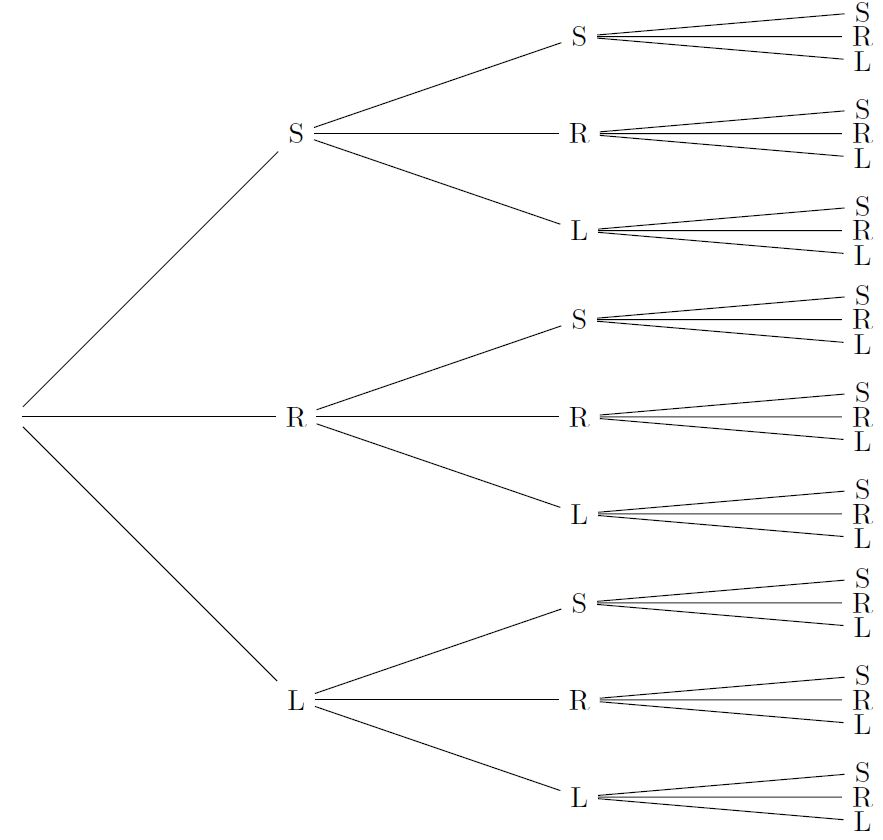
\includegraphics[width=12.26in]{./figures/vehicles} 

}

\caption{A tree diagram representing the choices for the three vehicles}\label{fig:tree}
\end{figure}

\begin{enumerate}
\def\labelenumi{\alph{enumi})}
\item
  \(0.35^3\)
\item
  \(0.45^3+0.2^3+0.35^3\)
\item
  LLR can be rearranged in \(3\) ways: LLR, LRL, RLL. \(3\times 0.45^2 \times 0.2\).
\item
  SRL can be rearranged in \(3!\) ways. \(3!\times 0.35 \times 0.45 \times 0.2\).
\item
  LLR or LLS. Each can be rearranged in \(3\) ways, then these are mutually exclusive outcomes so we can add the probabilities. \[3\times 0.45^2 \times 0.2 + 3\times 0.45^2 \times 0.35\].
\end{enumerate}

\hypertarget{conditional-probability}{%
\section{Conditional Probability}\label{conditional-probability}}

We will consider the following examples to motivate the definition of conditional probability.

\begin{example}

The number of insurance claims in the previous \(12\) months is cross tabulated with whether the driver involved was a young driver.

\begin{longtable}[]{@{}crrr@{}}
\toprule
& Under 25 & 25 and over & Total\tabularnewline
\midrule
\endhead
No claim & 225 & 725 & 950\tabularnewline
Claim & 25 & 25 & 50\tabularnewline
& 250 & 750 & 1000\tabularnewline
\bottomrule
\end{longtable}

\end{example}

The insurance company is interested in the claim rate. Overall the claim rate is,

\[\text{P}(\text{Claim})=\frac{50}{1000} = 0.05\]

An estimate for the probability of a driver claiming on the insurance is then \(1\) in \(20\).

However this figure hides a substantial difference in the claim rates for young and older drivers.

If we consider the \(250\) young drivers separately we have,

\[\text{P}(\text{Claim}|\text{Under}\ 25)=\frac{25}{250} = 0.1.\]
Whereas for the \(750\) older drivers we have,

\[\text{P}(\text{Claim}| 25 \ \text{and over})=\frac{25}{750} = 0.03.\]

The notation \(|\) is read `given that' and is a conditional statement. The conditional probabilities show that the claim rate is much higher for the younger drivers. One can compute the ratio of these probabilities to see how many times higher it is, \(0.1/0.03 \approx 3.3\), so this is just over three times higher. This relative risk scoring is common in medical statistics.

\begin{example}
\protect\hypertarget{exm:cancer}{}\label{exm:cancer}Consider the following data from a study on male lung cancer patients carried out in \(1950\) in the UK. This was one of the earliest applications of epidemiology - the use of statistics to study disease patterns in populations.

\begin{longtable}[]{@{}crrr@{}}
\toprule
& Non-smoker & Smoker & Total\tabularnewline
\midrule
\endhead
Lung cancer & 2 & 647 & 649\tabularnewline
No lung cancer & 27 & 620 & 647\tabularnewline
& 29 & 1267 & 1296\tabularnewline
\bottomrule
\end{longtable}

Calculate the relative risk of having lung cancer for a smoker compared to a non-smoker.

\emph{solution}

\[\text{P}(\text{Lung cancer}|\text{Smoker}) = \frac{647}{1267}\]

\[\text{P}(\text{Lung cancer}|\text{Non-smoker}) = \frac{2}{29}\]

There is \(\approx 7.4\) times higher relative risk of lung cancer in smokers.
\end{example}

These examples motivate the definition of conditional probability.

\begin{definition}[conditional probability]
The \textbf{\emph{conditional probability}} \(\text{P}(A|B)\) of an event \(A\) given another event of non-zero probability \(B\) is given by,

\[\text{P}(A|B) = \frac{\text{P}(A\cap B)}{\text{P}(B)}.\]
\end{definition}

One should verify that the fraction on the left is precisely how the conditional probability was calculated in the previous two examples.

\begin{theorem}
The conditional probability \(\text{P}(A|B)\) satisfies Kolmogorov's definition of probability.
\end{theorem}

\begin{proof}
Not lectured or examined, but here for completeness.

Firstly need to check \(P(A|B)\in[0,1]\). We have \(P(A|B) \geq 0\) because \(P(A\cap B)\geq0\) and \(P(B)>0\).

Because the intersection of \(B\) with another set is contained in \(B\), we have \(A\cap B \subseteq B\), and so
\[P(A\cap B) \leq P(B).\]
And dividing through by \(P(B)\) gives \(P(A|B) \leq 1\).

Secondly, \[P(\Omega|B) = \frac{P(\Omega \cap B)}{P(B)} = \frac{P(B)}{P(B)}=1.\]

Lastly, any given any two disjoint \(A_1\),\(A_2\) such that \(A_1\cap A_2 = \varnothing\).

We have that

\begin{align}
P(A_1\cup A_2 |B) &= \frac{P((A_1\cup A_2)\cap B)}{P(B)} \\
&= \frac{P((A_1\cap B)\cup (A_2\cap B))}{P(B)} \\
&= \frac{P(A_1\cap B)}{P(B)} + \frac{P(A_2\cap B)}{P(B)} \\
&= P(A_1|B) + P(A_2|B)
\end{align}
\end{proof}

\begin{example}
Note that \(P(A|B) \neq P(B|A)\). Revisiting the driver's example gives,

\begin{longtable}[]{@{}crrr@{}}
\toprule
& Under 25 & 25 and over & Total\tabularnewline
\midrule
\endhead
No claim & 225 & 725 & 950\tabularnewline
Claim & 25 & 25 & 50\tabularnewline
& 250 & 750 & 1000\tabularnewline
\bottomrule
\end{longtable}

\[\text{P}(\text{Claim}|\text{Under}\ 25)=0.1.\]
However,
\[\text{P}(\text{Under}\ 25|\text{Claim})=\frac{25}{50} = 0.5\]
\end{example}

\begin{theorem}
Two events \(A\) and \(B\) are \emph{independent} if and only if
\[\text{P}(A|B) = \text{P}(A) \ \text{ or } \ \text{P}(B|A) = \text{P}(B)\]
In other words, conditioning on either event does not affect the probability of the other event occurring.
\end{theorem}

\begin{proof}
Using the definition of conditional probability,
\[\text{P}(A\cap B) = \text{P}(A|B)\text{P}(B)=\text{P}(B|A)\text{P}(A)\]
If
\[\text{P}(A|B) = \text{P}(A) \ \text{ or } \ \text{P}(B|A) = \text{P}(B),\]
substituting this in the former yields
\[\text{P}(A\cap B) = \text{P}(A)\text{P}(B), \]
which is the definition of independence.
Conversely if two events are independent, we have
\[\text{P}(A|B) = \frac{\text{P}(A\cap B)}{\text{P}(B)} = \frac{\text{P}(A)\text{P}(B)}{\text{P}(B)} = \text{P}(A), \]
and likewise for \(\text{P}(B|A)\).
\end{proof}

When constructing tree diagrams the probabilities involved are usually conditional probabilities as there is a natural progression through the tree from left to right conditioning on what happened previously. In the diagram below, the events \(A\) and \(B\) may not be independent.

\begin{figure}

{\centering 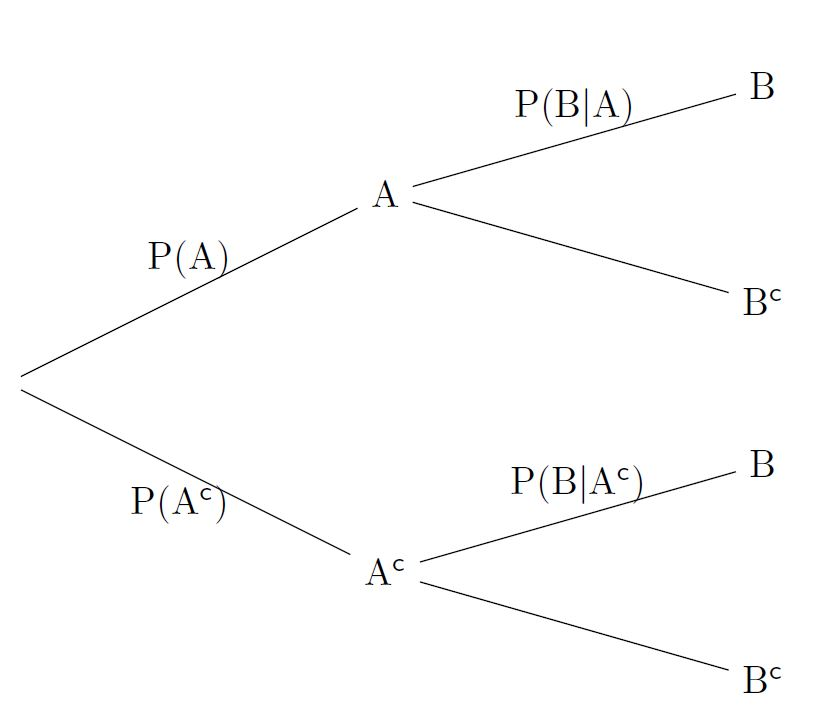
\includegraphics[width=11.31in]{./figures/condtree} 

}

\caption{The second level of branches represent the conditional probabilities of B given A or its complement, which may be different numbers}\label{fig:tree2}
\end{figure}

\begin{example}
Jon always goes to campus by bike or takes a tram. If one day he goes to campus by bike, the probability that he goes to campus by tram the next day is \(0.4\). If one day he goes to campus by tram, the probability that he goes to campus by bike the next day is \(0.7\).
Given that Jon goes to campus on Monday by tram, find the probability that he takes a tram to campus on Wednesday.

\emph{solution}

This may be solved by considering a tree diagram with levels for Tuesday and Wednesday. The probabilities in the question are \(\text{P}(\text{tram} \ |\ \text{bike})=0.4\) and \(\text{P}(\text{bike} \ |\ \text{tram})=0.7\).
Monday's journey is done. Possible sequences are `tram then tram', or `bike then tram'. These are mutually exclusive outcomes. The calculation is then

\[0.3^2+0.7\times 0.4 = 0.37\].
\end{example}

Surveys with questions of a sensitive or delicate nature often result in respondents missing that question or lying about their answers. Conditional probability can be used to mask the awkward question and find the proportion who would answer a certain way.

\begin{example}
A company want to find the proportion of employees who have ever called in sick to work, when in fact they were not sick. The boss asks each employee to toss a coin and hide the result.

If the result is \textbf{\emph{heads}}, the employee should answer the question `is your age an odd number?'.

If the result is \textbf{\emph{tails}}, they should answer `Have you ever taken a day off when you should not have?'.

Because the boss does not know which question people are answering, the employees can answer truthfully.

Suppose that \(40\%\) of employees mark `yes' as their answer. Let,

\[p= \text{P}(\text{taken a day off} \ | \ \text{tails})\]
Assume that ages are randomly distributed so that the chance of an even or odd number of years old is \(0.5\). How can we find \(p\)?
\end{example}

\emph{solution}

One can draw a tree diagram.

\begin{figure}

{\centering 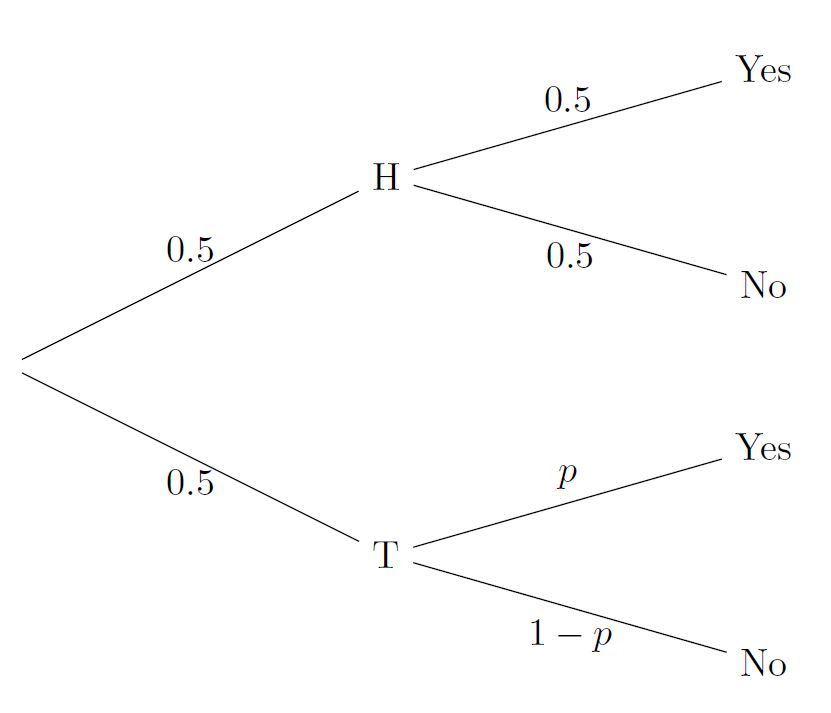
\includegraphics[width=11.54in]{./figures/survey} 

}

\caption{The outcomes of the survey.}\label{fig:tree3}
\end{figure}

The overall probability of answering `yes' is \(0.25+0.5p\), and in the survey \(40\%\) answered `yes'. We then have

\[0.25+0.5p = 0.4, \]
and hence \(p=0.3\). This means we can estimate that \(30\%\) of employees have taken a day of when they were not supposed to.

\hypertarget{bayes-theorem}{%
\section{Bayes Theorem}\label{bayes-theorem}}

\begin{example}
There are two coins in a bag. One coin is fair, while the other has heads on both sides (a double-header).

A coin is selected from the bag at random, and the selected coin is flipped three times. Unfortunately the coin which was selected is unknown to us.

On each of three flips the coin comes up heads.

Without doing any calculations, how likely do you think it is to be the unfair coin?
\end{example}

\emph{solution}

Let
\(A =\left\{ \text{The double-header is selected} \right\}\) and
\(B =\left\{ \text{The coin lands heads up three times in a row} \right\}\)

\begin{figure}

{\centering 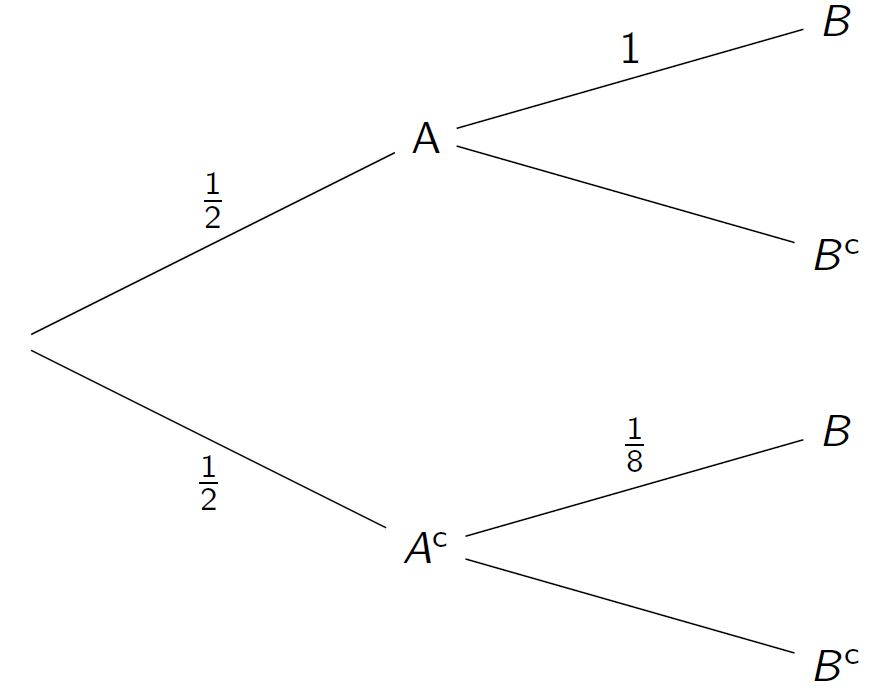
\includegraphics[width=12.38in]{./figures/doubleheader} 

}

\caption{A tree diagram for the double headed coin example.}\label{fig:tree4}
\end{figure}

One can use the tree diagram to find \(8/9\).

We can generalise this picture and come up with a formula for the conditional probability called Bayes' formula.

\begin{figure}

{\centering 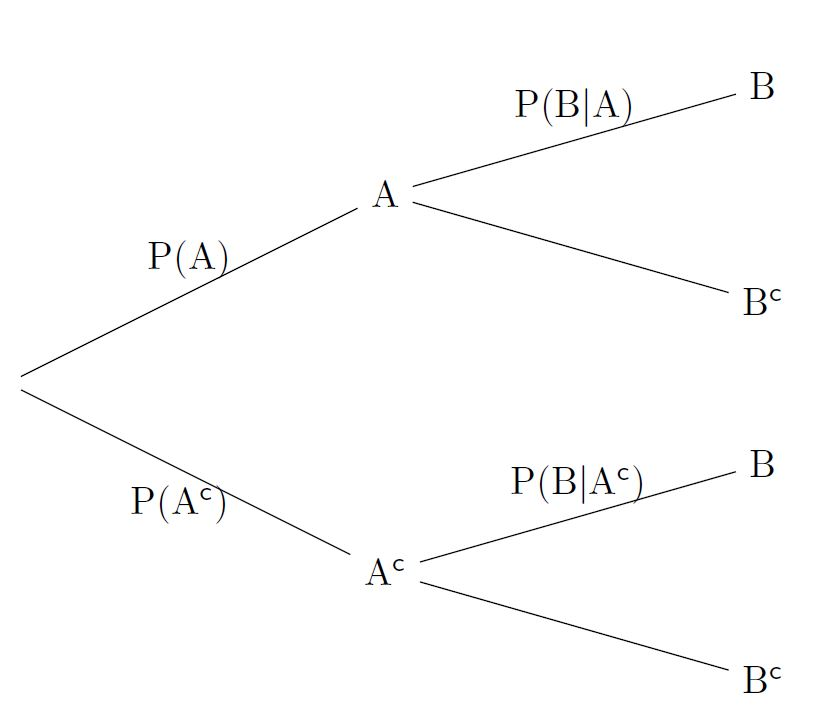
\includegraphics[width=11.31in]{./figures/condtree} 

}

\caption{Tree showing Bayes' formula}\label{fig:tree5}
\end{figure}

\[P(A|B) = \frac{P(A\cap B)}{P(B)} = \frac{P(A)P(B|A)}{P(A)P(B|A)+P(A^{\mathsf{c}})P(B|A^{\mathsf{c}})}\]

Previously, \(A_1=A\) and \(A_2 = A^{\mathsf{c}}\) are disjoint and their union gives the entire sample space. This situation is called a \emph{partition}.

This can be extended to a partition of \(n\) events \(A_1,A_2, \dots , A_n\).

\begin{definition}
A collection of events \(A_1, A_2, \dots , A_n\) is a \textbf{\emph{partition}} if their union is the entire sample space, that is \emph{exhaustive}, and they are mutually exclusive. That is

\begin{enumerate}
\def\labelenumi{\roman{enumi})}
\item
  \(\Omega = A_1 \cup A_2 \cup \dots \cup A_n\).
\item
  \(A_1 \cap A_2 \cap \dots \cap A_n = \varnothing\)
\end{enumerate}

Any event and its complement form a partition.
\end{definition}

Here is a picture of a partition:

\begin{figure}

{\centering 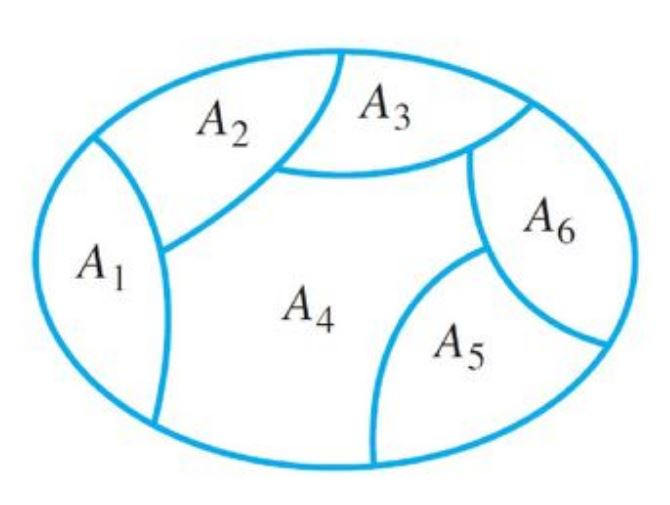
\includegraphics[width=9.31in]{./figures/partition} 

}

\caption{An example partition with six sets.}\label{fig:partition}
\end{figure}

We can now extend the concept of conditional probability to a general situation in which we condition on the event of at least one event of a partition.

\begin{theorem}[Law of Total Probability]
Suppose we have a partition \(A_1, A_2, \dots , A_n\) of the sample space \(\Omega\). Then for any event \(B \subseteq \Omega\), we have

\[\text{P}(B) =P(A_1)P(B|A_1)+ \dots + P(A_n)P(B|A_n) \]
\end{theorem}

An intuitive proof is to imagine a tree diagram with \(n\) branches for each of the \(A_i\) in the first layer, then \(B\) and \(B^{\mathsf{c}}\) in the next layer. As you multiply along all the branches the ways that \(B\) can occur you end up with the sum in the RHS.

\begin{theorem}[Bayes' Theorem]
Suppose we have a partition \(A_1, A_2, \dots , A_n\) of the sample space \(\Omega\). Then the conditional probability of any one event of the partition \(A_k\) for some \(k\), given any other event \(B\) can be written as,

\[\text{P}(A_k |B) = \frac{\text{P}(B|A_k)\text{P}(A_k)}{\sum^{n}_{i=1}\text{P}(B|A_i)P(A_i)}\]
\end{theorem}

\begin{proof}
Note that \(\text{P}(A_k\cap B) = \text{P}(B|A_k)\text{P}(A_k)\),

and that the denominator is \$\text{P}(B) using the law of total probability.
\end{proof}

\begin{example}
A company produces electrical components using three shifts. During the first shift \(50%
\) of components are produced, with \(20\%\) and \(30\%\) being produced during shifts \(2\) and \(3\) respectively. The proportion of defective components produced during shift \(1\) is \(6\%\). For shifts \(2\) and \(3\) the proportions are \(8\%\) and \(12\%\) respectively.

\begin{enumerate}
\def\labelenumi{\alph{enumi})}
\item
  Find the percentage of defective components.
\item
  If a component is defective, what is the probability that it came from shift \(3\)?
\end{enumerate}

\emph{solution}

Let \(D\) be the event that the component is defective and \(S_1,S_2,S_3\) denotethat it was produced during shifts \(1,2\) or \(3\) respectively.

\begin{enumerate}
\def\labelenumi{\alph{enumi})}
\item
  Use the theorem of total probability, as follows:
  \begin{align}
  \text{P}(D)  &= \text{P}(D|S_1)P(S_1)+\text{P}(D|S_2)\text{P}(S_2)+\text{P}(D|S_3)\text{P}(S_3) \\
  &= 0.06\times 0.5 + 0.08\times 0.2 + 0.12\times 0.3 \\
  &= 0.082
  \end{align}
\item
  Using Bayes' theorem,
\end{enumerate}

\[\text{P}(S_3|D) = \frac{\text{P}(D|S_3)\text{P}(S_3)}{\text{P}(D)}\]
The denominator was worked out in part a), this gives \(\frac{0.12\times 0.3}{0.082}=0.439\).
\end{example}

Bayes' theorem allows us to update the probability of an event in the light of new evidence. This is in fact the main practical use of the theorem, and leads to a whole branch of Bayesian Statistics.

\begin{example}
Gary is suspected of committing a crime. The evidence so far points to a probability of guilt being \(0.9\). To `prove his innocence' Gary undergoes a lie detector test, which has a \(70\%\) accuracy rate. The test will say positive to indicate guilt, and negative to indicate not guilty. The test is such that
\[\text{P}(\text{Positive}|\text{Guilty}) = 0.7\]
\[\text{P}(\text{Negative}|\text{Innocent})=0.7\]

If Gary's test comes back \textbf{\emph{negative}}, what is then the probability of his guilt?

\emph{solution}

One can directly apply Bayes' theorem.
\[\text{P}(\text{Guilt}|\text{Negative})=\frac{\text{P}(\text{Negative}|\text{Guilt})\text{P}(\text{Guilt})}{\text{P}(\text{Negative}|\text{Guilt})\text{P}(\text{Guilt})+\text{P}(\text{Negative}|\text{Innocent})\text{P}(\text{Innocent})}\]
and so
\[\text{P}(\text{Guilt}|\text{Negative})=\frac{0.3\times 0.9}{0.3\times 0.9 \ + \ 0.7\times 0.1}=0.794 \ \text{(3 d.p.)}\]
\end{example}

Beware of having extreme prior beliefs, for no evidence can then change your mind. Believing something to be true \(100\%\) or \(0\%\), will mean that no reason or evidence will change this position.

\begin{example}[Cromwell's Rule]
If we believe Gary is \(100\%\) guilty at the start then
\[\text{P}(\text{Guilt}|\text{Negative})=\frac{0.3\times 1}{0.3\times 1 \ + \ 0.7\times 0}=1\]
So we would still believe Gary to be \(100\%\) guilty.

If we believe Gary is \(0\%\) guilty at the start then
\[\text{P}(\text{Guilt}|\text{Negative})=\frac{0.3\times 0}{0.3\times 0 \ + \ 0.7\times 1}=0\]
So we would still believe Gary to be \(0\%\) guilty.
\end{example}

As educated people we should always consider the opposing opinion and update our own beliefs according to the evidence available. If you have a strong opinion about something, consider what would change your mind. Always leave some room to doubt yourself, because you could be wrong.

\hypertarget{exercises-week-2}{%
\section{Exercises Week 2}\label{exercises-week-2}}

\begin{exercise}

I toss a fair coin and roll a die.
a) Are these events independent?

\begin{enumerate}
\def\labelenumi{\alph{enumi})}
\setcounter{enumi}{1}
\tightlist
\item
  What is the probability I obtain a head and a \(6\)?
\end{enumerate}

\end{exercise}

\begin{exercise}

A torch uses two batteries in series. Each battery works with probability \(0.95\), independently of the other. Work out the probability that:

\begin{enumerate}
\def\labelenumi{\alph{enumi})}
\item
  The torch will work.
\item
  Both batteries fail
\item
  Only one of the batteries will work.
\end{enumerate}

\end{exercise}

\begin{exercise}
Whether a student gets up on time depends on whether or not he has remembered to set his alarm the night before. Some \(90\%\) of the time he remembers, the other \(10\%\) he forgets. When the clock is set, he will get up on time \(95\%\) of occasions. If it is not set, the chance he will oversleep is \(35\%\). Use a tree diagram to find the probability that he will oversleep.
\end{exercise}

\begin{exercise}
The following data shows the distribution of male and female students on various degree courses at a university.

\begin{longtable}[]{@{}cccc@{}}
\toprule
& Accountancy & Economics & Finance\tabularnewline
\midrule
\endhead
Male & 330 & 360 & 90\tabularnewline
Female & 120 & 390 & 60\tabularnewline
\bottomrule
\end{longtable}

Suppose a student is selected at random. Find the probability that they are,

\begin{enumerate}
\def\labelenumi{\alph{enumi})}
\item
  female
\item
  studying Economics
\item
  male and studying Economics
\item
  male given that they are studying Economics
\item
  female given that they are studying Economics
\item
  studying Economics given that they are female
\end{enumerate}

Are the events `student is male' and `studying Economics' independent?
\end{exercise}

\begin{exercise}

The following table shows the lung cancer data for females in the same \(1950\) study given in example \ref{exm:cancer}.

\begin{longtable}[]{@{}crrr@{}}
\toprule
& Non-smoker & Smoker & Total\tabularnewline
\midrule
\endhead
Lung cancer & 19 & 41 & 60\tabularnewline
No lung cancer & 32 & 28 & 60\tabularnewline
& 51 & 69 & 120\tabularnewline
\bottomrule
\end{longtable}

\begin{enumerate}
\def\labelenumi{\alph{enumi})}
\item
  Calculate the relative risk for female smokers compared to non-smokers.
\item
  Can you suggest any reason for the difference in the figures between males and females?
\end{enumerate}

\end{exercise}

\begin{exercise}

Two electrical components \(X\) and \(Y\) have probabilities of working \(\frac{3}{4}\) and \(\frac{7}{8}\), respectively. They also function independently of each other. Two devices \(D_1\) and \(D_2\) are constructed. In \(D_1\), \(X\) and \(Y\) are in series, and in \(D_2\) they are wired in parallel.

\begin{enumerate}
\def\labelenumi{\alph{enumi})}
\item
  \begin{enumerate}
  \def\labelenumii{(\roman{enumii})}
  \tightlist
  \item
    Find the probability that \(D_1\) works.
  \end{enumerate}
\end{enumerate}

\begin{enumerate}
\def\labelenumi{(\roman{enumi})}
\setcounter{enumi}{1}
\tightlist
\item
  Find the probability that \(D_2\) works.
\end{enumerate}

\begin{enumerate}
\def\labelenumi{\alph{enumi})}
\setcounter{enumi}{1}
\tightlist
\item
  Suppose that \(D_1\) works, find the probability that;
\end{enumerate}

\begin{enumerate}
\def\labelenumi{(\roman{enumi})}
\tightlist
\item
  \(X\) is working.
\item
  Only \(X\) is working.
\item
  both \(X\) and \(Y\) are working.
\end{enumerate}

\begin{enumerate}
\def\labelenumi{\alph{enumi})}
\setcounter{enumi}{2}
\tightlist
\item
  Suppose that \(D_2\) works, find the probability that;
\end{enumerate}

\begin{enumerate}
\def\labelenumi{(\roman{enumi})}
\tightlist
\item
  \(X\) is working.
\item
  Only \(X\) is working.
\item
  both \(X\) and \(Y\) are working.
\end{enumerate}

\end{exercise}

\begin{exercise}

An urn contains two green balls and three red bals. Supose two balls will be drawn at random one after another and without replacement. Draw a tree diagram, and find the probability that:

\begin{enumerate}
\def\labelenumi{\alph{enumi})}
\item
  a green ball appears on the first draw.
\item
  a green ball appears in the second draw.
\end{enumerate}

\end{exercise}

\begin{exercise}
The following table shows the \emph{fear factor} for children attending the dentist, cross tabulated with the School age of the child.

\begin{longtable}[]{@{}lccc@{}}
\toprule
& Infant & Primary & Secondary\tabularnewline
\midrule
\endhead
Afraid & 0.12 & 0.08 & 0.05\tabularnewline
Not afraid & 0.28 & 0.25 & 0.22\tabularnewline
\bottomrule
\end{longtable}

For a child selected at random define the events; \(A = \{ \text{The child is afraid} \}\),

with \(N\) being not afraid, and \(I\),\(P\) and \(S\) being the School age in the obvious fashion.

Calculate the following probabilities,

\begin{enumerate}
\def\labelenumi{\alph{enumi})}
\item
  \(\text{P}(A)\), \(\text{P}(N)\), \(\text{P}(A\cup I)\).
\item
  \(\text{P}(A| I)\) and \(\text{P}(I| A)\).
\item
  \(\text{P}(A| S)\) and \(\text{P}(N| S)\) - what do you notice about these two probabilities?
\end{enumerate}

Are \(A\) and \(I\) independent?
\end{exercise}

\begin{exercise}
A survey by an electrical retailer determines that \(40\%\) of customers who seek advice from sales staff by an appliance and only \(20\%\) who do not seek advice buy an appliance. If \(30\%\) of customers seek advice, what is the probability that a customer entering the warehouse buys an appliance?
\end{exercise}

\begin{exercise}

Four cards are drawn at random without replacement from a deck of \(52\) cards. What is the probability that the sequence is:

\begin{enumerate}
\def\labelenumi{\alph{enumi})}
\item
  \(\heartsuit\) \(\heartsuit\) \(\spadesuit\) \(\clubsuit\)
\item
  \(\heartsuit\) \(\heartsuit\) \(\spadesuit\) \(\spadesuit\)
\end{enumerate}

\end{exercise}

\begin{exercise}

A student comes back from a night at the pub with a bunch of keys, only one of which works. They try one key at random in the lock and discard it if it doesn't fit.

\begin{enumerate}
\def\labelenumi{\alph{enumi})}
\tightlist
\item
  Suppose the bunch contains \(2\) keys. Find the probability they open the door on
\end{enumerate}

\begin{enumerate}
\def\labelenumi{(\roman{enumi})}
\item
  the first attempt
\item
  the second attempt
\end{enumerate}

\begin{enumerate}
\def\labelenumi{\alph{enumi})}
\setcounter{enumi}{1}
\item
  Repeat for a bunch of three keys being successul at the first, second and third attempts.
\item
  Suppose now that the bunch contains \(n\) keys. Find the probability that the door is opened on the \(r^{\text{th}}\) attempt (where \(1\leq r \leq n\)).
\end{enumerate}

\end{exercise}

\begin{exercise}
To ascertain the proportion of people who have had a sexually transmitted infection, the following survey pocedure was used on \(1000\) individuals.

They were asked to think of the day of the week their most recent birthday fell on.

If their last birthday was on a Monday, Tuesday or Wednesday they were to answer the question `Have you every had a sexually transmitted infection?'.

If their last birthday was on any other day of the week, they were to answer the question `Is your age an even number?'.

In the survey \(290\) people answered `yes'. Assuming that ages and birthdays are uniformly distributed, can you estimate the proportion of people who have had a sexually transmitted infection?
\end{exercise}

\begin{exercise}
Suppose two events \(A\) and \(B\) are independent. Show that \(A\) and \(B^{\mathsf{c}}\) are also independent. Show also that \(A^{\mathsf{c}}\) and \(B^{\mathsf{c}}\) are independent.
\end{exercise}

\begin{exercise}

Forty percent of new employees hired by a large company have a degree. Seventy percent of employees with degrees are promoted within two years.Of those without degrees, only \(30\%\) arepromoted within two years.

\begin{enumerate}
\def\labelenumi{\alph{enumi})}
\item
  What is the probability that a new empoyee will be promoted?
\item
  If an employee has been promoted, what is the probability that they have a degree?
\end{enumerate}

\end{exercise}

\begin{exercise}
A bag contains \(3\) coins; two are normal unbiased coins while the third is double headed. A coin is chosen at random from the bag and tossed. The coin is tossed \(4\) times and came up heads each time. What is the probability that it is the double header?
\end{exercise}

\begin{exercise}
Approximately \(25\%\) of males over \(50\) have some form of heart problem. A clinic has observed that males with a heart problem are three times more likely to be smokers as males with no heart problem. What is the probability that a male over \(50\) has a heart problem given that he is a smoker?
\end{exercise}

\begin{exercise}

Cage A contains five hens with disease and six hens without disease. Cage B contains two diseased hens and five hens without the disease. Two hens are chosen at random from cage A and transferred to cage B. A hen is now chosen at random from cage B and found to be diseased. Find the probability that the two hens that were transferred were,

\begin{enumerate}
\def\labelenumi{\alph{enumi})}
\item
  both diseased
\item
  both without disease.
\end{enumerate}

\end{exercise}

\hypertarget{drv}{%
\chapter{Discrete Random Variables}\label{drv}}

In most practical situations in which we encounter uncertainty, the random outcome of interest is a numerical quantity. This could be the number of minutes you end up waiting for that bus, how much you win on the lottery this week, or even the number of times you try to catch a fly with chopsticks before you eventually manage to do so.

\hypertarget{random-variables}{%
\section{Random Variables}\label{random-variables}}

In this chapter you will learn the concept of a discrete random variable.

\begin{example}
Suppose we roll two dice and find the sum of the numbers on the two dice. Let \(X\) be the sum of the numbers on the two dice. We know the sample space here is:
\[\Omega = \{ (n_1,n_2) : n_1,n_2 \in \mathbb{N}, \ 1 \leq n_1 , n_2 \leq 6 \},\]
Given an outcome \((n_1,n_2)\), the `variable' \(X\) takes a particular whole numbered value from \(x=2, \dots , 12\). We have seen that these particular values are not equally likely.
\end{example}

\begin{definition}
A \textbf{\emph{random variable}} \(X\) is a set function which maps the potential outcomes of a statistical experiment to (some subset of) the real number line.

A random variable is written with a capital letter (here \(X\)), and the particular values it takes are written with a lowercase of the same letter (here \(x\)). The probability that \(X\) takes a particular value is written \(\text{P}(X=x)\).
\end{definition}

Just as with data analysis there is a difference between \emph{discrete} and \emph{continuous} random variables. One can think of \emph{discrete} random variables arising from a process which involves counting and can take integer values. The \emph{continuous} random variables can be thought of as arising from a measuring process.

\begin{example}
Let \$R = \$ result of spinning a roulette wheel. The roulette wheel can take particular values
\[\Omega = \{0,1,2, \dots,36\}.\]
In number ranges from 1 to 10 and 19 to 28, odd numbers are red and even are black. In ranges from 11 to 18 and 29 to 36, odd numbers are black and even are red. There is a green pocket numbered 0 (zero). Then \(R\) is a discrete random variable, as it takes only particular discrete values.

Let \(T =\) the time spent waiting for a bus. Here \(T\) could be any positive number from when you arrive at the bus stop (if it were time after the timetabled arrival time, it could be negative for an early bus). Then \(T\) is a continuous random variable.
\end{example}

We will consider discrete random variables first, but will study both types in this course.

\hypertarget{discrete-probability-distributions}{%
\section{Discrete probability distributions}\label{discrete-probability-distributions}}

In order to understand how a random variable is likely to behave, and thus be able to predict its possible future values, we clearly need to consider the probability with which it will take on particular values. This set of probability values is known as a probability distribution. We will develop the theory with some examples.

\begin{definition}
The \textbf{\emph{distribution}} function, also known as a \textbf{\emph{probability mass function}}, of a random variable \(X\) is the function that outputs the probability of \(X\) attaining any particular value. That is,

\[f(x) = \text{P}(X=x)\]
In some texts, or if there are two variables in play, we may also write the variable in subscript \(f_X(x)\) to be clear to which mass function we are referring.
\end{definition}

\begin{example}[discrete uniform distribution]

Consider rolling a fair die and let the discrete random variable \(X\) be the score observed on the die. We know that the probability of getting any of the particular values in the set \(\{1,2, \dots 6\}\) is \(\frac{1}{6}\) and this is the probability distribution. We may tabulate the values as follows

\begin{longtable}[]{@{}cllllll@{}}
\toprule
\begin{minipage}[b]{0.28\columnwidth}\centering
\(x\)\strut
\end{minipage} & \begin{minipage}[b]{0.09\columnwidth}\raggedright
1\strut
\end{minipage} & \begin{minipage}[b]{0.09\columnwidth}\raggedright
2\strut
\end{minipage} & \begin{minipage}[b]{0.09\columnwidth}\raggedright
3\strut
\end{minipage} & \begin{minipage}[b]{0.09\columnwidth}\raggedright
4\strut
\end{minipage} & \begin{minipage}[b]{0.09\columnwidth}\raggedright
5\strut
\end{minipage} & \begin{minipage}[b]{0.09\columnwidth}\raggedright
6\strut
\end{minipage}\tabularnewline
\midrule
\endhead
\begin{minipage}[t]{0.28\columnwidth}\centering
\(\text{P}(X=x)\)\strut
\end{minipage} & \begin{minipage}[t]{0.09\columnwidth}\raggedright
\(\frac{1}{6}\)\strut
\end{minipage} & \begin{minipage}[t]{0.09\columnwidth}\raggedright
\(\frac{1}{6}\)\strut
\end{minipage} & \begin{minipage}[t]{0.09\columnwidth}\raggedright
\(\frac{1}{6}\)\strut
\end{minipage} & \begin{minipage}[t]{0.09\columnwidth}\raggedright
\(\frac{1}{6}\)\strut
\end{minipage} & \begin{minipage}[t]{0.09\columnwidth}\raggedright
\(\frac{1}{6}\)\strut
\end{minipage} & \begin{minipage}[t]{0.09\columnwidth}\raggedright
\(\frac{1}{6}\)\strut
\end{minipage}\tabularnewline
\bottomrule
\end{longtable}

\end{example}

Alternatively we may use a formula:
\begin{equation*}
  f(x)=\begin{cases}
    \frac{1}{6}, & \text{if } x = 1, 2, \dots , 6.\\
    0 & \text{otherwise}.
  \end{cases}
\end{equation*}

Or a graph:

\begin{figure}

{\centering 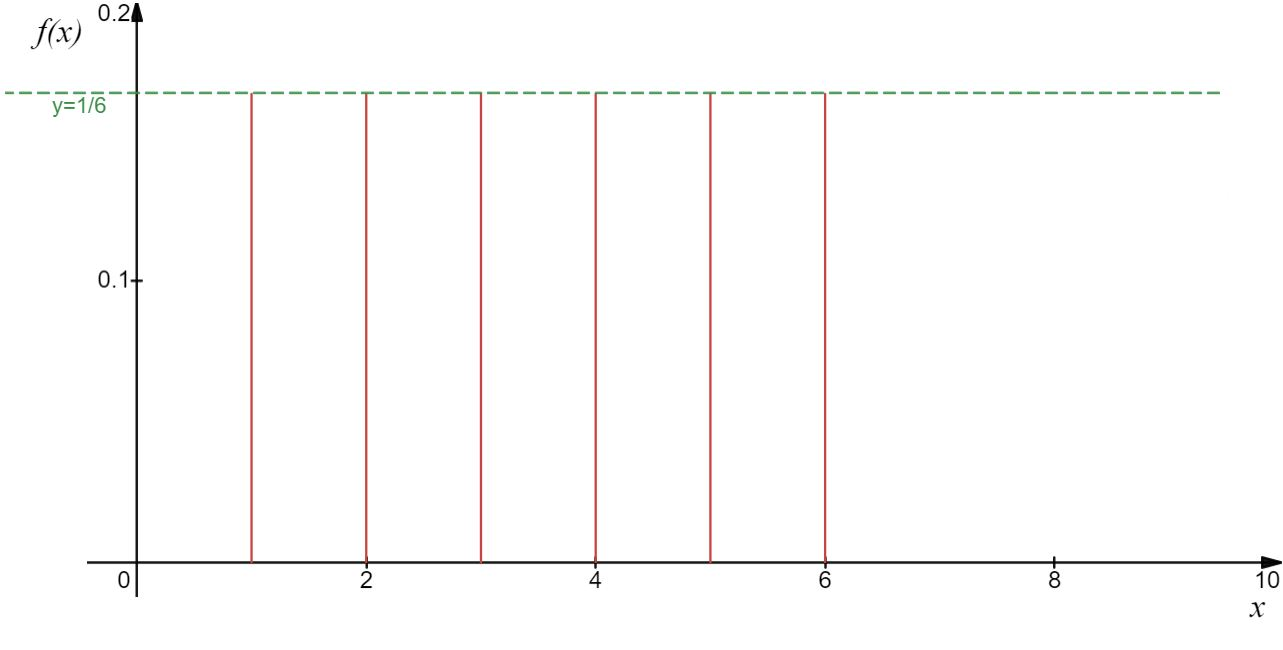
\includegraphics[width=0.75\linewidth]{./figures/uni_pdf} 

}

\caption{Probability mass function for a fair die}\label{fig:uniformdice}
\end{figure}

Clearly the graph is a very useful way to visualise how the probability is distributed. You can also see why this is called a discrete \emph{uniform} distribution - it's because the values are all the same.

Some questions to consider:

\begin{itemize}
\item
  Suppose your die had \(n\) sides, where \(n\) is some whole number greater than \(1\), and the faces numbered \(1,2,\dots n\). What does the distribution look like now?
\item
  Can you represent the distribution in each of the three ways above?
\end{itemize}

\begin{example}[Urn problem]
An urn contains five balls numbered \(1\) to \(5\). Two balls are drawn simultaneously.

\begin{enumerate}
\def\labelenumi{\arabic{enumi}.}
\item
  Let \(X\) be the larger of the two numbers.
\item
  Let \(Y\) be the sum of the two numbers.
\end{enumerate}

Find the probability distributions of \(X\) and \(Y\).

\emph{solution}

\begin{enumerate}
\def\labelenumi{\arabic{enumi}.}
\tightlist
\item
  We proceed as follows by enumerating all the possibilities and noting that there are \(^5C_2=10\) ways of drawing the balls from the urn. Note here that as the balls are drawn simultaneously, order does not matter here.
\end{enumerate}

To find the distribution of \(X\) one can list the outcomes systematically by the largest value.

\begin{longtable}[]{@{}cccccc@{}}
\toprule
\(x\) & & & & & \(\text{P}(X=x)\)\tabularnewline
\midrule
\endhead
2 & \((1,2)\) & & & & \(\frac{1}{10}\)\tabularnewline
3 & \((1,3)\) & \((2,3)\) & & & \(\frac{2}{10}\)\tabularnewline
4 & \((1,4)\) & \((2,4)\) & \((3,4)\) & & \(\frac{3}{10}\)\tabularnewline
5 & \((1,5)\) & \((2,5)\) & \((3,5)\) & \((4,5)\) & \(\frac{4}{10}\)\tabularnewline
\bottomrule
\end{longtable}

\begin{enumerate}
\def\labelenumi{\arabic{enumi}.}
\setcounter{enumi}{1}
\tightlist
\item
  To find the distribution of \(Y\) one can list the outcomes systematically by the sum.
\end{enumerate}

\begin{longtable}[]{@{}cccc@{}}
\toprule
\(y\) & & & \(\text{P}(Y=y)\)\tabularnewline
\midrule
\endhead
3 & (1,2) & & \(\frac{1}{10}\)\tabularnewline
4 & (1,3) & & \(\frac{1}{10}\)\tabularnewline
5 & (1,4) & (2,3) & \(\frac{2}{10}\)\tabularnewline
6 & (1,5) & (2,4) & \(\frac{2}{10}\)\tabularnewline
7 & (2,5) & (3,4) & \(\frac{2}{10}\)\tabularnewline
8 & (3,5) & & \(\frac{1}{10}\)\tabularnewline
9 & (4,5) & & \(\frac{1}{10}\)\tabularnewline
\bottomrule
\end{longtable}

In either case you should check that each individual probability is between \(0\) and \(1\) and that over all possible particular values the sum is \(1\).
\end{example}

\begin{example}[a geometric distribution]
\protect\hypertarget{exm:archer}{}\label{exm:archer}An archer hits a target rather randomly. Let's suppose that each time he takes aim \(\text{P}(\text{Hit})=\frac{1}{4}\), and so the complement \(\text{P}(\text{Miss})=\frac{3}{4}\). Let \(Y\) be the number of attempts required until he hits the target. Find the distribution of \(Y\).
\end{example}

\emph{solution}

We can consider the number of attempts separately.

\(Y=1\), first attempt is a hit, so \(\text{P}(Y=1)=\frac{1}{4}.\)

\(Y=2\), first attempt is a miss, second is a hit, so
\[\text{P}(Y=2)=\frac{3}{4}\times \frac{1}{4} = \frac{3}{16}.\]

\(Y=3\), first attempt is a miss, second is a miss, and third is a hit so
\[\text{P}(Y=3)=\frac{3}{4}\times \frac{3}{4}\times \frac{1}{4} = \frac{9}{64}.\]
\(Y=4\), the sequence is miss, miss, miss then hit:
\[\text{P}(Y=3)=\frac{3}{4}\times \frac{3}{4}\times \frac{3}{4}\times \frac{1}{4} = \frac{27}{256}.\]
And so on.

Notice that for the archer to hit the target on the \(y^{\text{th}}\) attempt, he must have missed on each of the previous \(y-1\) attempts, and so there is a formula for the mass function as follows.

\begin{equation*}
  f(Y=y)=\begin{cases}
    \left( \frac{3}{4} \right)^{y-1}\frac{1}{4} \ , & \text{if } y = 1, 2, 3, \dots \\
    \ 0 \ & \text{otherwise}.
  \end{cases}
\end{equation*}

Clearly these probabilities are quickly getting very small - you may recognise these terms as being in a geometric sequence with common ration \(\frac{3}{4}\).

A graph of this distribution looks like:

\begin{figure}

{\centering 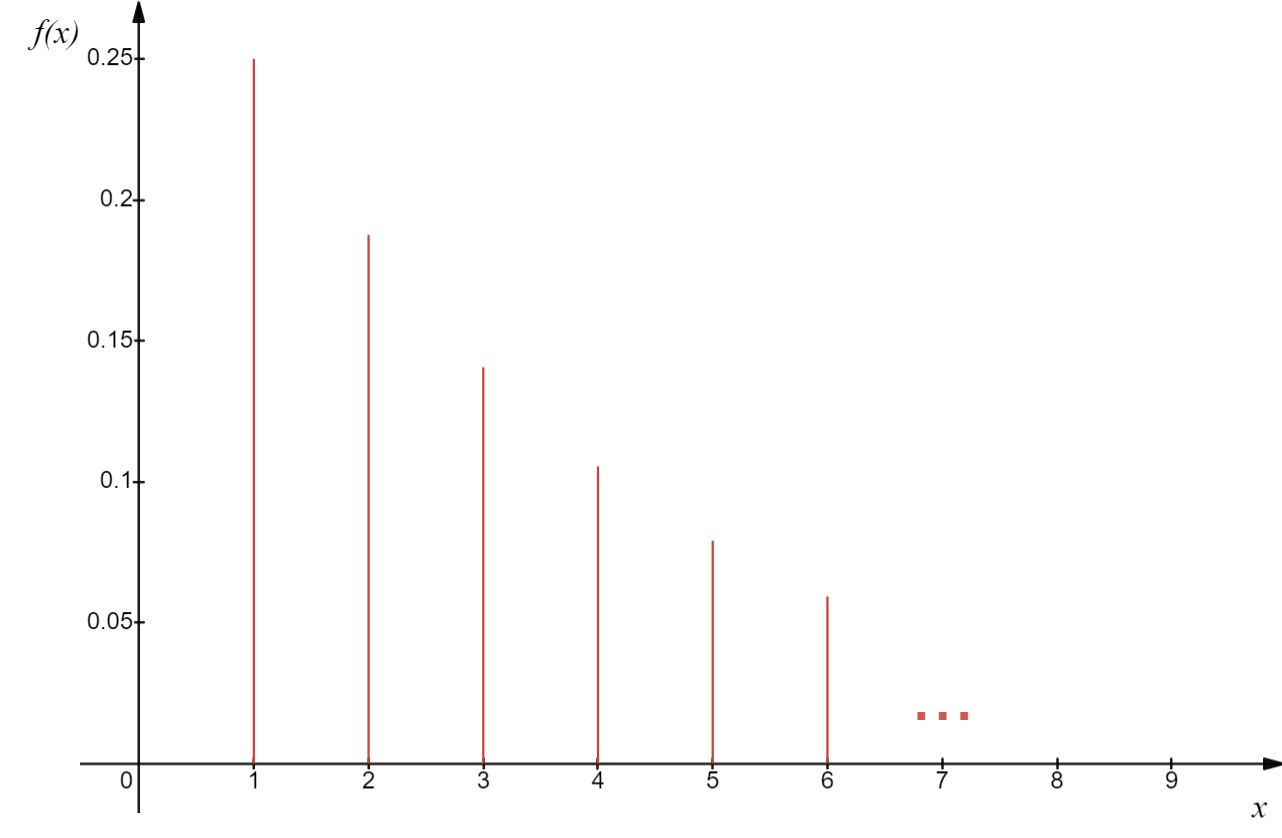
\includegraphics[width=0.75\linewidth]{./figures/geo_pdf} 

}

\caption{A geometric distribution}\label{fig:geomdriving}
\end{figure}

The choice of \(\frac{1}{4}\) is infact arbitrary. In general you can have `success' probability \(\pi\) and `failure' probability \(1-\pi\).

\begin{definition}
A random variable \(X\) representing the number of independent trials until the first success follows a geometric distribution with success probability \(\pi\), written as \(X \thicksim \text{Geom}(\pi)\), defined by the probability mass function

\begin{equation*}
  f(x)=\begin{cases}
    \left( 1-\pi \right)^{x-1}\pi , & x = 1, 2, 3, \dots \\
    \ 0 \ & \text{otherwise}.
  \end{cases}
\end{equation*}
\end{definition}

Of course the trials for the archer are arguably not independent - why?

\hypertarget{properties-of-probability-mass-functions}{%
\section{Properties of probability mass functions}\label{properties-of-probability-mass-functions}}

For a random variable \(X\) with probability distribution \(f(x)\) we have the following two properties:

\begin{enumerate}
\def\labelenumi{\arabic{enumi}.}
\item
  The probability of any particular value is between \(0\) and \(1\). That is,
  \[ 0 \leq f(x) \leq 1, \ \forall x\]
\item
  The probabilities sum to unity. That is,
\end{enumerate}

\[ \sum_{x} f(x)= 1\]

Probability distributions can be represented in a variety of different ways. In practice we use tables of distributions or use computer functions to evaluate them.

In R we can use the following functions to evaluate the probabilities from example \ref{exm:archer}.

\begin{Shaded}
\begin{Highlighting}[]
\NormalTok{y <-}\StringTok{ }\KeywordTok{dgeom}\NormalTok{(}\DataTypeTok{x =} \DecValTok{1}\OperatorTok{:}\DecValTok{4}\NormalTok{, }\CommentTok{#these are the particular values 1,2,3 and 4}
           \DataTypeTok{prob =} \DecValTok{1}\OperatorTok{/}\DecValTok{4}\NormalTok{ ) }\CommentTok{#This is the probability of success}
\NormalTok{y}
\end{Highlighting}
\end{Shaded}

\begin{verbatim}
## [1] 0.18750000 0.14062500 0.10546875 0.07910156
\end{verbatim}

\begin{Shaded}
\begin{Highlighting}[]
\CommentTok{#You can output these as fractions using the MASS library}
\NormalTok{MASS}\OperatorTok{::}\KeywordTok{fractions}\NormalTok{(y)}
\end{Highlighting}
\end{Shaded}

\begin{verbatim}
## [1]    3/16    9/64  27/256 81/1024
\end{verbatim}

The important function is \(\texttt{dgeom()}\), the \(\texttt{d}\) stands for distribution and \(\texttt{geom}\) for the geometric distribution.

Another way to represent a probability distribution is as a cumulative sum.

\begin{definition}[Cumulative distribution function]
Given a random variable \(X\) and its probability mass function \(f(x)\), the cumulative distribution function (abbreviated CDF) denoted with a capital letter \(F(x)\) is defined as the sum of the probabilities less than or equal to the value \(x\). That is,

\[ F(x) = \text{P}(X\leq x) = \sum_{t\leq x}f(t)\]
\end{definition}

\begin{example}[another urn problem]
Consider the setup previously where two balls numbered \(1\) through \(5\) are drawn and the maximum of two numbers is taken.
We found the probability distribution to be,

\begin{longtable}[]{@{}cc@{}}
\toprule
\(x\) & \(\text{P}(X=x)\)\tabularnewline
\midrule
\endhead
2 & \(\frac{1}{10}\)\tabularnewline
3 & \(\frac{2}{10}\)\tabularnewline
4 & \(\frac{3}{10}\)\tabularnewline
5 & \(\frac{4}{10}\)\tabularnewline
\bottomrule
\end{longtable}

Work out the CDF \(F(x)\).

\emph{solution}

If \(x<2\) we have \(F(x)=0\).
If \(2\leq x < 3\) we have \(F(x) = \frac{1}{10}\).
If \(3\leq x < 4\) we have \(F(x) = \frac{1}{10} + \frac{2}{10}\).
If \(4\leq x < 5\) we have \[F(x) = \frac{1}{10} + \frac{2}{10} + \frac{3}{10}.\]
If \(5\leq x\) we have \[F(x) = \frac{1}{10} + \frac{2}{10} + \frac{3}{10} + \frac{4}{10}.\]

Altogether,

\begin{equation*}
  F(x)=\begin{cases}
  0  \ \ \ \ \ \ \ \ \ \ \   x<2 \\
  \frac{1}{10} \  \  2\leq x < 3 \\
  \frac{3}{10} \ \  3\leq x < 4 \\
  \frac{6}{10} \ \ \ 4\leq x < 5 \\
  1 \ \ \  \ \ \  5\leq x
  \end{cases}
\end{equation*}
\end{example}

\begin{example}
The CDF of a geometric distribution is given by
\[F(x) = 1- (1-\pi)^{x}.\]
\end{example}

\emph{solution}

\[F(x) = \sum_{t\leq x}f(t)\]
Sum from \(t=1\) to \(t=x\).

\[  = \pi + \pi(1-\pi) + \pi(1-\pi)^2 + \dots +  \pi(1-\pi)^{x-1} \]
You might recognise a geometric series here, with \(a=\pi\) and \(r=(1-\pi)\), so this can be collected as:

\[F(x) = \frac{\pi (1-(1-\pi)^x)}{1-(1-\pi)} \]
Evaluating the denominator and cancelling gives the result.

The CDF is more useful than the mass function since if we are given the CDF we can calculate the mass function directly as the difference.

\[f(x) = F(x)-F(x-1)\]

\begin{example}
Calculate \(f(4)\) given the CDF

\begin{equation*}
  F(x)=\begin{cases}
  0  \ \ \ \ \ \ \ \ \ \ \   x<2 \\
  \frac{1}{10} \  \  2\leq x < 3 \\
  \frac{3}{10} \ \  3\leq x < 4 \\
  \frac{6}{10} \ \ \ 4\leq x < 5 \\
  1 \ \ \  \ \ \  5\leq x
  \end{cases}
\end{equation*}

\emph{solution}

\(f(4) = F(4)-F(3) = \frac{6}{10}-\frac{3}{10} = \frac{3}{10}\)
\end{example}

Due to the fact that the mass function can be calculated from the CDF, statistical tables often prioritise tabulating the CDF for various different types of distribution.

We finish this section with an example of how this theory may be used in applied calculations.

\begin{example}

Assuming the archer's attempts to hit a target follows a geometric distribution with success parameter \(\frac{1}{4}\) calculate the probability that he

\begin{enumerate}
\def\labelenumi{\arabic{enumi}.}
\item
  Hits on the \(10^{\text{th}}\) attempt.
\item
  Takes fewer than \(4\) attempts to hit the target.
\item
  Takes at least \(8\) attempts to hit the target.
\item
  Takes between \(4\) and \(8\) attempts inclusive.
\end{enumerate}

\end{example}

\emph{solution}

Let \(Y\) be the number of attempts to hit the target. We know that

\[f(y) = \left( \frac{3}{4} \right) ^{y-1}\frac{1}{4}\]

and

\[ F(y) = 1- \left(1-\frac{1}{4}\right)^y = 1-\left( \frac{3}{4}\right)^y.\]

\begin{enumerate}
\def\labelenumi{\arabic{enumi}.}
\item
  \(\text{P}(Y=10) = f(10) = \left( \frac{3}{4}\right)^9\times \frac{1}{4} = 0.0188\) (\(3\) s.f.).
\item
  \(\text{P}(Y<4) = \text{P}(Y\leq 3) = F(3) =1 - \left( \frac{3}{4}\right)^3 = 0.578\), (\(3\) s.f.).
\item
  Using the complement, \(\text{P}(Y\geq 8) = 1 - \text{P}(Y\leq 7)\). Now using the CDF:
\end{enumerate}

\[1-F(7) = 1- \left( 1-\left(\frac{3}{4}\right)^7\right) = 0.134.\]

\begin{enumerate}
\def\labelenumi{\arabic{enumi}.}
\setcounter{enumi}{3}
\tightlist
\item
  Rewrite the required range as a difference of two CDF values as follows:
\end{enumerate}

\[\text{P}(4\leq Y\leq 8) = \text{P}(Y\leq 8) - \text{P}(Y\leq 3)\]

\[ = F(8) - F(3)\]

\[ = \left[ 1-\left(\frac{3}{4}\right)^8\right] -  \left[ 1-\left(\frac{3}{4}\right)^3\right]\]
\[ = 0.322\]
You should be careful when evaluating the CDF to ensure that you have the correct values in the given inequality. A small diagram or list can be invaluable here.

\hypertarget{mean-variance-and-moments}{%
\section{Mean, variance and moments}\label{mean-variance-and-moments}}

The mean and variance of a random variable essentially mirror the definitions of mean and variance for samples.The mean or expected value is the \emph{average} value of the variable if it were observed repeatedly. The variance indicates the likely spread of values of the variable.

\begin{example}
If you toss a coin \(2\) times how many heads would you expect to turn up?

\emph{solution}

Your would expect \(1\) intuitively. Let \(X\) be the number of heads.
The outcomes are \((T,T),(H,T),(T,H),(H,H)\). The average number of heads is then

\[ \frac{0+1+1+2}{4} = 1\]
We can relate this to the probability of each number of heads. We have,

\[\text{P}(X=0) = \frac{1}{4}\]
\[\text{P}(X=1) = \frac{2}{4}\]
\[\text{P}(X=2) = \frac{1}{4}\]

The sum of the possible \(x\) values weighted by the probability is:
\[0\times \frac{1}{4} + 1\times \frac{2}{4} + 2\times \frac{1}{4} = 1.\]
\end{example}

\begin{definition}
The \textbf{\emph{expectation}}, or \textbf{\emph{expected value}} of a random variable \(X\) is defined as the sum of the possible values of the random variable weighted by the probability of that value.

\[ \text{E}[X] = \sum_x x\times\text{P}(X=x)\]
This is just a number once it is calculated is called the \textbf{\emph{mean}}, and so is written as a constant \(\text{E}[X]=\mu\) to omit the random quantity \(X\).

The expected value of any function of a discrete random variable \(g(X)\) is defined similarly by
\[ \text{E}[X] = \sum_x g(x)\times\text{P}(X=x)\]
\end{definition}

\begin{definition}
The \textbf{\emph{variance}} of a random variable \(X\) is defined as:

\[ \text{Var}[X] = \text{E}[(X-\mu)^2]\]
\end{definition}

The following is a very useful in practice for actually computing the variance.

\begin{theorem}
Given a random variable \(X\) we have that the variance is equal to the difference between the expectation of \(X^2\) and the squared expectation of \(X\). That is,

\[ \text{Var}[X]=\text{E}[X^2]-\text{E}[X]^2 \]
\end{theorem}

We omit the proof for now and see some examples, leaving this for the interested reader.

\begin{proof}
The expectation is a sum, so behaves linearly. By definition,

\[\text{Var}[X] = \text{E}[(X-\mu)^2]\]
Expanding out the bracket on the inside gives,
\[ = \text{E}[X^2 - 2\mu X +\mu^2] \]
Using linearity,

\[= \text{E}[X^2]-2\mu\text{E}[X]+\mu^2.\]
\[= \text{E}[X^2]-2\mu^2+\mu^2.\]
Hence the result.
\end{proof}

\begin{example}

A discrete random variable \(X\) representing the score on a loaded die has the following probability mass function.

\begin{longtable}[]{@{}cllllll@{}}
\toprule
\begin{minipage}[b]{0.28\columnwidth}\centering
\(x\)\strut
\end{minipage} & \begin{minipage}[b]{0.09\columnwidth}\raggedright
1\strut
\end{minipage} & \begin{minipage}[b]{0.09\columnwidth}\raggedright
2\strut
\end{minipage} & \begin{minipage}[b]{0.09\columnwidth}\raggedright
3\strut
\end{minipage} & \begin{minipage}[b]{0.09\columnwidth}\raggedright
4\strut
\end{minipage} & \begin{minipage}[b]{0.09\columnwidth}\raggedright
5\strut
\end{minipage} & \begin{minipage}[b]{0.09\columnwidth}\raggedright
6\strut
\end{minipage}\tabularnewline
\midrule
\endhead
\begin{minipage}[t]{0.28\columnwidth}\centering
\(\text{P}(X=x)\)\strut
\end{minipage} & \begin{minipage}[t]{0.09\columnwidth}\raggedright
\(\frac{1}{21}\)\strut
\end{minipage} & \begin{minipage}[t]{0.09\columnwidth}\raggedright
\(\frac{2}{21}\)\strut
\end{minipage} & \begin{minipage}[t]{0.09\columnwidth}\raggedright
\(\frac{3}{21}\)\strut
\end{minipage} & \begin{minipage}[t]{0.09\columnwidth}\raggedright
\(\frac{4}{21}\)\strut
\end{minipage} & \begin{minipage}[t]{0.09\columnwidth}\raggedright
\(\frac{5}{21}\)\strut
\end{minipage} & \begin{minipage}[t]{0.09\columnwidth}\raggedright
\(\frac{6}{21}\)\strut
\end{minipage}\tabularnewline
\bottomrule
\end{longtable}

Calculate:

\begin{enumerate}
\def\labelenumi{\alph{enumi})}
\item
  \(\text{E}[X]\)
\item
  \(\text{E}[X^2]\)
\item
  \(\text{Var}[X]\)
\item
  \(\text{E}[e^X]\)
\end{enumerate}

\end{example}

\emph{solution}

\begin{enumerate}
\def\labelenumi{\alph{enumi})}
\tightlist
\item
  Using the definition of expectation:
\end{enumerate}

\[ \text{E}[X] = 1\times \frac{1}{21}+2\times \frac{2}{21}+3\times \frac{3}{21}+4\times \frac{4}{21}+5\times \frac{5}{21}+6\times \frac{6}{21},\]
\[ = 4.33 \ \ \ (3 \ \text{s. f.})\]
Compared to a fair die, the mean of the loaded die is higher.

\begin{enumerate}
\def\labelenumi{\alph{enumi})}
\setcounter{enumi}{1}
\tightlist
\item
  \[ \text{E}[X^2] = 1^2\times \frac{1}{21}+2^2\times \frac{2}{21}+3^2\times \frac{3}{21}+4^2\times \frac{4}{21}+5^2\times \frac{5}{21}+6^2\times \frac{6}{21},\]
\end{enumerate}

\[ = 21\]

\begin{enumerate}
\def\labelenumi{\arabic{enumi}.}
\setcounter{enumi}{2}
\tightlist
\item
  The variance is then,
\end{enumerate}

\[\text{Var}[X]=\text{E}[X^2]-\mu^2 = 21-(4.33\dots)^2= 2.22 \ \ \ (3 \ \text{s. f.})\]
4. \(e^X\) is just a function of \(X\).

\[ \text{E}[X] = e^1\times \frac{1}{21}+e^2\times \frac{2}{21}+e^3\times \frac{3}{21}+e^4\times \frac{4}{21}+e^5\times \frac{5}{21}+e^6\times \frac{6}{21},\]

\[ = 164.622 \ (3 \ \text{d. p.}) \]

\begin{example}[expected profit]
Consider the following game. A spinning wheel is divided into three equal sections numbered \(1\), \(2\) and \(3\). You pay £\(1\) to play the game, and you have to guess the number that will show when the wheel is spun. If you guess correctly, you get £\(2\). If you do not then you get nothing. What is the expected profit from playing the game?

\emph{solution}

The profit is the winnings minus the stake. Let the profit be the random variable \(X\). The distribution of \(X\) is:

\begin{longtable}[]{@{}cllllll@{}}
\toprule
\(x\) & -1 & 1 & & & &\tabularnewline
\midrule
\endhead
\(\text{P}(X=x)\) & \(\frac{2}{3}\) & \(\frac{1}{3}\) & & & &\tabularnewline
\bottomrule
\end{longtable}

\[\text{E}[X] = -1 \times \frac{2}{3} + 1 \times \frac{1}{3} = -\frac{1}{3}\]
So we would expect on average to make a loss playing this game. For any gambling game to be profitable for the house, it is necessary that the expectation of the players winnings be negative.
\end{example}

\begin{example}
Let \(X\) be a random variable whose value is a constant, that is the particular values it can take are all the same, \(x=a\). Show that \(\text{E}[X]=a\) and \(\text{Var}[X]=0\)

\emph{solution}

\[\text{E}[X]=\sum_{x}x\times\text{P}(X=x)= \sum a\times\text{P}(X=a)=a\times \sum \text{P}(X=a) = a \times 1 = a\]

For the variance,

\[ \text{Var}[X] = \text{E}[(X-\mu)^2]=\text{E}[(a-a)^2]=0 \]
\end{example}

We will now proceed to find the mean and variance of a Geometric distribution. We will need a fact about series first.

\begin{proposition}
Suppose \(|r|<1\) and recall the infinite geometric series is given by the following formula:

\[g(r) = \sum_{k=0}^{\infty}ar^{k} = \frac{a}{1-r}\]
For a convergent series such as this we can differentiate term by term with respect to \(r\), and equate this to what we would get from differentiating the RHS likewise. Doing so results in the following two formulae:

\[g'(r) = \sum_{k=0}^{\infty}akr^{k-1} = \frac{a}{(1-r)^2}\]

\[g''(r) = \sum_{k=0}^{\infty}ak(k-1)r^{k-2} = \frac{2a}{(1-r)^3}\]
\end{proposition}

\begin{theorem}
Let \(X\) be a random variable which follows a geometric distribution, \(X \thicksim \text{Geom}(\pi)\), then we have:

\[\text{E}[X] = \frac{1}{\pi}\]
and
\[ \text{Var}[X]=\frac{1-\pi}{\pi^2}\]
\end{theorem}

\begin{proof}
By definition,
\[\text{E}[X] = \sum_{x=1}^{\infty}x(1-\pi)^{x-1}\pi\]
\[ = \pi + 2\pi(1-\pi) + 3\pi(1-\pi)^2+4\pi(1-\pi)^3+ \dots \]
The latter sum can be seen as \(g'(1-\pi)\), with \(a=\pi\). Using the RHS result from the previous proposition we have,
\[\text{E}[X] = \frac{\pi}{[1-(1-\pi)]^2} = \frac{1}{\pi}\]
For the variance we first find the expectation of a function of \(X\) called a factorial moment.

\[\text{E}[X(X-1)] = \sum_{x=1}^{\infty}x(x-1)\pi(1-\pi)^{x-1}\]
\[ = (1-\pi)\sum_{x=2}^{\infty}x(x-1)\pi(1-\pi)^{x-2}\]
The infinite series turns out to be \(g''(1-\pi)\) with \(a=\pi\). Substituting this in gives,

\[\text{E}[X(X-1)]=(1-\pi)\frac{2\pi}{[1-(1-\pi)]^3} = \frac{2(1-\pi)}{\pi^2}.\]
Now we can use this to find the variance as follows,

\[\text{Var}[X] = \text{E}[X^2]-\text{E}[X]^2 \]
\[ = \text{E}[X(X-1)]+\text{E}[X]-\text{E}[X]^2 \]
\[ = \frac{2(1-\pi)}{\pi^2} + \frac{1}{\pi} - \frac{1}{\pi^2} \]
\[ = \frac{1-\pi}{\pi^2}\]
as required.
\end{proof}

If you are given two random variables \(X\) and \(Y\) a \emph{linear combination} means an expression of the form \(aX+bY\).

\begin{theorem}[Linear Combinations]
For any random variables \(X\) and \(Y\) and constants \(a\) and \(b\) we have that the expectation of a linear combination is a linear combination of the expectations.

\[\text{E}[aX\pm bY] = a\text{E}[X]\pm b\text{E}[Y]\]
However the variance is a nonlinear sum of the variances.\\
\[\text{Var}[aX\pm bY] = a^2\text{Var}[X]+b^2\text{Var}[Y] \]
\end{theorem}

\begin{proof}
This is omitted, but follows from properties of summations and mass functions.
\end{proof}

\begin{example}
Recall the loaded die had mass function given by,

\begin{longtable}[]{@{}cllllll@{}}
\toprule
\begin{minipage}[b]{0.28\columnwidth}\centering
\(x\)\strut
\end{minipage} & \begin{minipage}[b]{0.09\columnwidth}\raggedright
1\strut
\end{minipage} & \begin{minipage}[b]{0.09\columnwidth}\raggedright
2\strut
\end{minipage} & \begin{minipage}[b]{0.09\columnwidth}\raggedright
3\strut
\end{minipage} & \begin{minipage}[b]{0.09\columnwidth}\raggedright
4\strut
\end{minipage} & \begin{minipage}[b]{0.09\columnwidth}\raggedright
5\strut
\end{minipage} & \begin{minipage}[b]{0.09\columnwidth}\raggedright
6\strut
\end{minipage}\tabularnewline
\midrule
\endhead
\begin{minipage}[t]{0.28\columnwidth}\centering
\(\text{P}(X=x)\)\strut
\end{minipage} & \begin{minipage}[t]{0.09\columnwidth}\raggedright
\(\frac{1}{21}\)\strut
\end{minipage} & \begin{minipage}[t]{0.09\columnwidth}\raggedright
\(\frac{2}{21}\)\strut
\end{minipage} & \begin{minipage}[t]{0.09\columnwidth}\raggedright
\(\frac{3}{21}\)\strut
\end{minipage} & \begin{minipage}[t]{0.09\columnwidth}\raggedright
\(\frac{4}{21}\)\strut
\end{minipage} & \begin{minipage}[t]{0.09\columnwidth}\raggedright
\(\frac{5}{21}\)\strut
\end{minipage} & \begin{minipage}[t]{0.09\columnwidth}\raggedright
\(\frac{6}{21}\)\strut
\end{minipage}\tabularnewline
\bottomrule
\end{longtable}

Suppose you win \(W\) is an amount depending on the number that you roll on the loaded die.

If \(W = 3X-10\) find \(\text{E}[W]\) and \(\text{Var}[W]\)

\emph{solution}

\[\text{E}[W] = 3\times (4.333\dots) -10 = £3\]

\[\text{Var}[W] = 3^2\times(2.22\dots) = 19.99\dots = 20.0 \  (3 \ \text{s.f.})\]
\end{example}

\hypertarget{exercises-week-3}{%
\section{Exercises Week 3}\label{exercises-week-3}}

\begin{exercise}

An urn contains two yellow balls and three red balls. Three balls are drawn at random from the urn without replacement.

\begin{enumerate}
\def\labelenumi{\alph{enumi})}
\item
  Draw a tree diagram to represent the sample space for this experiment and find the probabilities of each outcome.
\item
  Let the random variable \(X\) denote the number of red balls drawn.
\item
  Write down the probability distribtion of \(X\).
\end{enumerate}

\begin{enumerate}
\def\labelenumi{\roman{enumi})}
\setcounter{enumi}{1}
\tightlist
\item
  Find the mean and variance of \(X\).
\end{enumerate}

\end{exercise}

\begin{exercise}

Let \(X\) be the value observed from rolling an \(8\)-sided die

\begin{enumerate}
\def\labelenumi{\alph{enumi})}
\item
  What is the probability distribution of \(X\).
\item
  Draw a graph of the probability distribution.
\item
  Find the mean and variance of \(X\).
\item
  Find the expected value of:
\item
  \(3X+5\)
\end{enumerate}

\begin{enumerate}
\def\labelenumi{\roman{enumi})}
\setcounter{enumi}{1}
\tightlist
\item
  \(\ln(X)\)
\end{enumerate}

\end{exercise}

\begin{exercise}

A game consists of tossing a coin until the first head appears. The score recorded is the number of tosses required.

\begin{enumerate}
\def\labelenumi{\alph{enumi})}
\item
  If the random variable \(Y\) is the number of tosses, what is the distribution of \(Y\)?
\item
  Write down the first \(6\) values of the probability distribution, and draw a sketch.
\item
  Find the mean and variance of \(Y\).
\end{enumerate}

\end{exercise}

\begin{exercise}

Two fair dice are rolled and the \emph{total} score observed.

\begin{enumerate}
\def\labelenumi{\alph{enumi})}
\item
  Write down the probability distribution of the total score.
\item
  Find the mean and variance of the total score.
\end{enumerate}

\end{exercise}

\begin{exercise}

Two fair dice are rolled and the \emph{maximum} score observed.

\begin{enumerate}
\def\labelenumi{\alph{enumi})}
\item
  Write down the probability distribution of the maximum score.
\item
  Find the mean and variance of the maximum score.
\end{enumerate}

\end{exercise}

\begin{exercise}

A fair coin is tossed three times. Let \(X\) be the number of heads in the tosses minus the number of tails.
a) Find the probability distribution of \(X\)

\begin{enumerate}
\def\labelenumi{\alph{enumi})}
\setcounter{enumi}{1}
\tightlist
\item
  Find the mean and variance of \(X\).
\end{enumerate}

\end{exercise}

\begin{exercise}

The game of simple \emph{Chuck-a-luck} is played by a single player against the house. The game is conducted as follows:

The player chooses any number between \(1\) and \(6\) inclusive and places a bet of £\(1\). The banker then rolls \(2\) fair dice. If the player's number occurs \(1\) or \(2\) times, he wins £\(1\) or £\(2\) respectively. If the player's numberdoes not appear on any of the dice, he loses his £\(1\) stake. Let the random variable \(X\) denote the player's winnings in the game.

\begin{enumerate}
\def\labelenumi{\alph{enumi})}
\item
  Find the probability mass function of \(X\).
\item
  Find the expected value of the winnings, \(\text{E}[X]\).
\end{enumerate}

\end{exercise}

\begin{exercise}

The random variable \(X\) has the following probability mass function:

\begin{longtable}[]{@{}cccccc@{}}
\toprule
\(x\) & 1 & 2 & 3 & 4 & 5\tabularnewline
\midrule
\endhead
\(\text{P}(X=x)\) & \(7c\) & \(5c\) & \(4c\) & \(3c\) & \(c\)\tabularnewline
\bottomrule
\end{longtable}

\begin{enumerate}
\def\labelenumi{\alph{enumi})}
\item
  Find the value of \(c\) which makes this a valid probability mass function.
\item
  Find \(\text{E}[X]\) and \(\text{Var}[X]\).
\end{enumerate}

\end{exercise}

\begin{exercise}

The random variable \(X\) has the following probability mass function:

\begin{longtable}[]{@{}cccccc@{}}
\toprule
\(y\) & 2 & 3 & 5 & 7 & 11\tabularnewline
\midrule
\endhead
\(\text{P}(Y=y)\) & \(\frac{1}{6}\) & \(\frac{1}{3}\) & \(\frac{1}{4}\) & \(a\) & \(b\)\tabularnewline
\bottomrule
\end{longtable}

and \(\text{E}[Y]=\frac{14}{3}\)

\begin{enumerate}
\def\labelenumi{\alph{enumi})}
\item
  Find the values of \(a\) and \(b\).
\item
  Find \(\text{Var}[Y]\).
\end{enumerate}

\end{exercise}

\begin{exercise}

A fair six-sided die has `\(1\)' on one face, `\(2\)' on two faces and `\(3\)' on the remaining three faces.

\begin{enumerate}
\def\labelenumi{\alph{enumi})}
\item
  Let \(Y\) denote the score on a single roll of the die. Tabulate the mass function and calculate the mean and variance of \(Y\).
\item
  Let \(X\) be the total score on two rolls of the die. Tabulate the mass function and calculate the mean and variance of \(X\).
\end{enumerate}

\end{exercise}

\begin{exercise}
An urn contains \(n\) balls numbered \(1\) to \(n\) from which two balls are drawn simultaneously. Find the probability distribution of \(X\), the larger of the two numbers drawn. Calculate the expected value of \(X\).
\end{exercise}

\begin{exercise}

\(A\) and \(B\) play a game that involves each rolling a fair die simultaneously. Let \(X\) be the absolute difference in their scores.

\begin{enumerate}
\def\labelenumi{\alph{enumi})}
\item
  Tabulate the probability mass function of \(X\).
\item
  Find the mean and variance of \(X\).
\item
  If the value of \(X\) is \(1\) or \(2\) then \(A\) wins. If \(X\) is \(3\),\(4\) or \(5\) then \(B\) wins. If \(X\) is zero then they roll again. Find the probability that \(A\) wins on the first go. Find the probability that \(A\) wins on the second go. Find the probability that \(A\) wins on the \(r^{\text{th}}\) go.
\item
  Find the probability that \(A\) wins.
\end{enumerate}

\end{exercise}

\begin{exercise}
A discrete random variable has the following mass function

\begin{equation*}
  f(y)=\begin{cases}
    \pi \ \ \ \ \ \ \ \ \ \  y = 1 \\
    1-\pi \ \  \ y = 0 .
  \end{cases}
\end{equation*}

Where \(0<\pi<1\).This is known as the Bernoulli distribution.Find \(\text{E}[Y]\) and \(\text{Var}[Y]\)
\end{exercise}

\hypertarget{exercises-for-feedback-1}{%
\subsection{Exercises for feedback}\label{exercises-for-feedback-1}}

\begin{exercise}

Scrabble tiles for the letters of the word EXERCISES are in a bag.

\begin{enumerate}
\def\labelenumi{\alph{enumi})}
\item
  A random tile is drawn, what is the probability that it is the letter is E?
\item
  Given that the letter that is drawn from the bag is a vowel, what is the probability that it is an E?
\item
  Explain how the two questions are different in your own words, and compare the size of the probabilities in either part.
\end{enumerate}

\end{exercise}

\begin{exercise}

There are \(40\) students in a Maths class, and each are given a number \(1\) to \(40\). Separately the numbers \(1-40\) are placed in a hat and mixed randomly. The teacher will give three random students a prize. Three numbers are selected from the hat without replacement. Before the numbers are drawn the teacher guesses three numbers and writes them on the board.

\begin{itemize}
\tightlist
\item
  Work out the probability of the teacher matching \(0\), \(1\), \(2\) or \(3\) of the numbers that are drawn from the hat.
\end{itemize}

On a different occasion, the teacher has \(5\) students in his tutor group. He wants to give two prizes to the Maths students, and one to his tutor group. He will draw two numbers from his hat, and separately he will draw one of the numbers \(1-5\) from his shoe (he only has one hat). Again he writes his prediction on the board before the selection.

\begin{itemize}
\tightlist
\item
  Work out the probability of the teacher predicting \(0\), \(1\) or \(2\) Maths students, but not getting the tutee correct, and the probability of predicting \(0\), \(1\) or \(2\) Maths students and getting the tutee correct.
\end{itemize}

\end{exercise}

\begin{exercise}

A fairground game is played with \(5\) dice. The player pays £1 to play, and for every \(6\) that appears on the dice the player is rewarded with £\(6\).

\begin{enumerate}
\def\labelenumi{\alph{enumi})}
\item
  Work out the probabilities of getting \(0\),\(1\),\(2\),\(\dots\),\(5\) sixes when rolling the five dice.
\item
  If \(X\) is the profit of for the player of this game, work out the expected profit \(\text{E}[X]\).
\item
  Work out also the variance \(\text{Var}[X]\).
\item
  Explain if you think this is a good game or not.
\end{enumerate}

\end{exercise}

\begin{exercise}[Extension / Challenge]
You play a game with a standard pack of \(52\) cards. You are dealt a hand of \(3\) cards. If your hand contains a pair, you get \(3\) points. If your hand contains \(3\) of a kind, you get \(10\) points. If your hand contains neither a pair nor \(3\) of a kind you lose a point. What is the expected number of points you will score in this game?
\end{exercise}

\hypertarget{binpois}{%
\chapter{Special discrete random variables}\label{binpois}}

In this chapter you should be able to recognise contexts in which Binomial distributions arise. Calculate binomial probabilities using formulae. Use binomial tables, calculators and R to look up probabilities.

\hypertarget{the-binomial-distribution}{%
\section{The Binomial Distribution}\label{the-binomial-distribution}}

The binomial distribution is one of the most important discrete distributions and finds application in a wide number of areas.

The example to have in mind is the following:

\begin{example}[coin tossing]

Suppose you toss a coin \(10\) times and count the number of heads that are observed.

\begin{itemize}
\item
  There is fixed number of trials, here \(10\), and so a maximal number of heads we can observe.
\item
  The coin is the same, and so the probability of heads is the same throughout the process. For a fair coin this is \(\frac{1}{2}\).
\item
  The coin tosses are independent. There is no physical reason why any previous outcome may make heads more or less likely on subsequent tosses.
\item
  There are only two outcomes for a coin toss: heads or tails.
\end{itemize}

\end{example}

The binomial distribution can be used to find probabilities whenever the following conditions are met:

\begin{itemize}
\item
  The probability of observing a success in a single experiment is a fixed quantity, that is the probability is a constant \(\text{P}(\text{success}) = \pi\). (P for constant probability)
\item
  The trials are independent. (I)
\item
  The number of experiments, or trials, is a fixed number and so there is a maximum value attainable. (N for maximum number)
\item
  There are only two outcomes.(T for two outcomes)
\end{itemize}

The list of assumptions underlying the binomial model above can be summarised in the mnemonic PINT.

Although you can check the mnemonic is satisfied, it may in practicebe easier in a given situation to make an analogy with the coin tossing example. In a particular context the number could well vary, as could the definition of `success'. For example, suppose you are considering how many out of a number of men over \(50\), will suffer a heart attack in the next year. Then a `success' is a heart attack!

\hypertarget{the-binomial-mass-function}{%
\section{The binomial mass function}\label{the-binomial-mass-function}}

\begin{example}
You throw five drawing pins in the air and note if they land pin up or pin down. How many ways can two of the pins land facing up and the others land face down?

Suppose the probability a single pin lands facing up is \(0.3\), what is the probability that exactly two land facing up?

\emph{solution}

Consider this problem as a word UUDDD, how many different words can be obtained by rearrangement? The number of ways of rearranging this is \(\frac{5!}{2!}{3!} = 10\).

Note that this is one of the choice numbers \(^5C_2\). We are choosing from \(5\) things, two to be face up and so the remaining ones to be face down.

For any choice of two pins we have the same calculation for the probability. That is, \(0.3^2 \times 0.7^3\).

Altogether the probability is \(^5C_2 \times 0.3^2 \times 0.7^3\).
\end{example}

We can derive the binomial mass function in a similar way as this example.

\begin{theorem}
Suppose the random variable \(X\) satisfies the conditions of a binomial random variable, so that there are \(n\) trials with success probability \(\pi\). The mass function is given by:
\[\text{P}(X=x) = {}^nC_x \pi^{x}(1-\pi)^{n-x}\]
\end{theorem}

\begin{proof}
If the \(n\) trials result in \(x\) successes, each with probability \(\pi\), there must have also been \(n-x\) failures each with probability \((1-\pi)\). Using independence, the probability of this happening is

\[\pi ^x (1-\pi)^{n-x} \]
There are a number of ways this can happen, equal to \(^nC_x\). Hence result.
\end{proof}

\begin{example}
\protect\hypertarget{exm:fourfairdice}{}\label{exm:fourfairdice}Suppose a fair die is rolled four times. What is the probability of getting,

\begin{enumerate}
\def\labelenumi{\alph{enumi})}
\item
  exactly one six?
\item
  at most \(1\) six?
\end{enumerate}

\emph{solution}

\begin{enumerate}
\def\labelenumi{\alph{enumi})}
\tightlist
\item
  A common mistake is \$ \frac{1}{6}\times \left( \frac{5}{6} \right)\^{}3\$. This is not correct - why? Because it can happen in \(^4C_1=4\) ways,
\end{enumerate}

\[4\times \frac{1}{6}\times \left( \frac{5}{6} \right)^3 = 0.386 \text{ (3 s.f.)}\]

\begin{enumerate}
\def\labelenumi{\alph{enumi})}
\setcounter{enumi}{1}
\tightlist
\item
  if \(X\) is the number of sixes, at most one means \(X \leq 1\). You could work this out by adding the two cases \(X=0\) and \(X=1\) together. One could calculate directly from the mass function as follows:
\end{enumerate}

\[^4C_0 \times \left( \frac{1}{6} \right)^0 \times \left( \frac{5}{6} \right)^4+ ^4C_1 \times \left( \frac{1}{6} \right)^1 \times \left( \frac{5}{6} \right)^3\]
Obtaining \(0.868\text{ (3 s.f.)}\).
\end{example}

Some examples of binomial probability distributions are given in the following figures.

\begin{figure}

{\centering 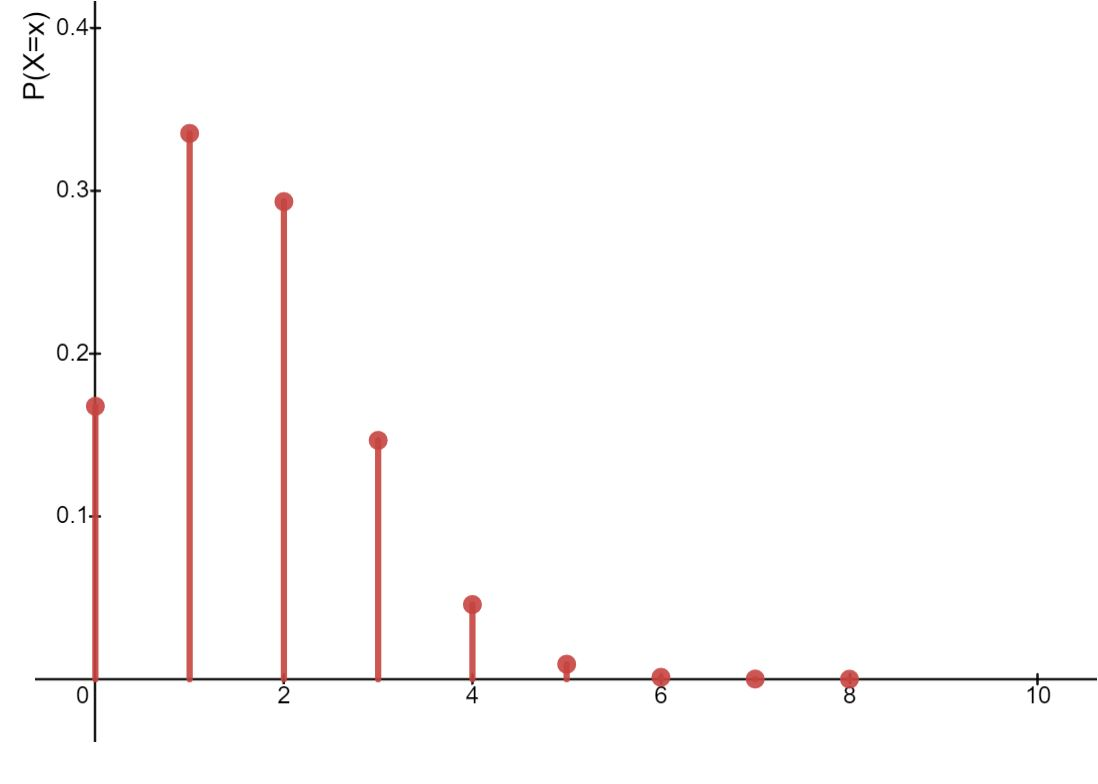
\includegraphics[width=0.75\linewidth]{./figures/binomial1} 

}

\caption{Probability mass function for B(9,0.2)}\label{fig:bin1}
\end{figure}

\begin{figure}

{\centering 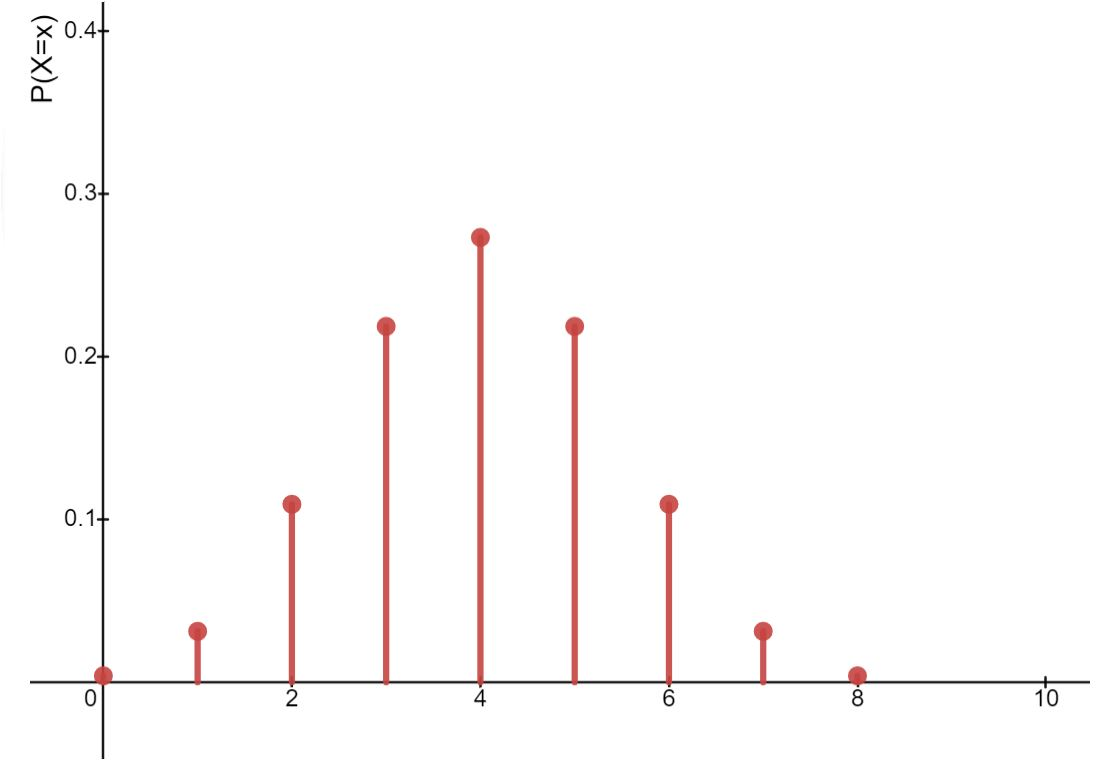
\includegraphics[width=0.75\linewidth]{./figures/binomial2} 

}

\caption{Probability mass function for B(8,0.5)}\label{fig:bin2}
\end{figure}

How can we account for the seemingly different shape?

If the success probability is close to \(0.5\) the distribution has a symmetrical shape, otherwise it is skewed.

\begin{example}
A train station has \(5\) self-service ticket machines. The probability of a machine not working at any time is \(0.15\). Let \(X\) be the number of machines not working.

\begin{enumerate}
\def\labelenumi{\alph{enumi})}
\tightlist
\item
  Comment on whether a binomial distribution is a suitable model for \(X\).
\end{enumerate}

Assuming a binomial distribution for X, evaluate the probability of the following number of machines not working.

\begin{enumerate}
\def\labelenumi{\alph{enumi})}
\setcounter{enumi}{1}
\item
  exactly \(2\).
\item
  at least \(4\).
\item
  at most \(2\).
\end{enumerate}

\emph{solution}

\begin{enumerate}
\def\labelenumi{\alph{enumi})}
\item
  Checking the mnemonic PINT here works. Here a `success' is a ticket machine not working. Independence might not hold if for example one machine not working caused the others to also fail somehow, but here the probability is the same \emph{at any time} including at a time when others have failed.
\item
  \(\text{P}(X=2) = ^5C_2 \times 0.15^2 \times (1-0.15)^{5-2} = 0.138\).
\item
  \(\text{P}(X\geq 4) = \text{P}(X=4) + \text{P}(X=5)\). Evaluating the formulae gives:
\end{enumerate}

\[= {}^5C_4 \times 0.15^4 \times (1-0.15)^{5-4}+ ^5C_5 \times 0.15^5 \times (1-0.15)^{5-5}\]
\[= 0.0022\]

\begin{enumerate}
\def\labelenumi{\alph{enumi})}
\setcounter{enumi}{3}
\tightlist
\item
  \(\text{P}(X\leq 2) = \text{P}(X=0) + \text{P}(X=1) + \text{P}(X=2)\). Again evaluating the formula for each term in the sum gives:
\end{enumerate}

\[= {}^5C_0 \times 0.15^0 \times (1-0.15)^{5-0}+ {}^5C_1 \times 0.15^1 \times (1-0.15)^{5-1}+ {}^5C_2 \times 0.15^2 \times (1-0.15)^{5-2}\]
\[ = 0.973 \]
\end{example}

Alternatively, if the number of cases to add is large enough to be tedious by hand calculation (here we only need to add a few cases together), one may consult statistical tables of the CDF.

Because the binomial distribution is so widely applied and is so important, almost every book of statistical tables will contain some pages of the binomial CDF. The tables used at MMU give probabilities for selected values of \(n\) and \(\pi\) in the form \(\text{P}(X\leq x)\). Any probability can be calculated from these tables using rules like the following:

\begin{itemize}
\item
  \(\text{P}(X\leq x)\), directly from table.
\item
  \(\text{P}(X\geq x) = 1- \text{P}(X\leq x-1)\), using complements.
\item
  \$\text{P}(X = x) = \text{P}(X\leq x) - \text{P}(X\leq x-1) \$, as with getting the mass function from the CDF in the usual way.
\end{itemize}

You can the probability of \(X\) lying in a range too, but one must be careful about whether the inequality is strict or not.

\begin{itemize}
\item
  \$\text{P}(a\leq X\leq b) = \text{P}(X\leq b) - \text{P}(X\leq a-1) \$
\item
  \$\text{P}(a\textless{} X\leq b) = \text{P}(X\leq b) - \text{P}(X\leq a) \$
\item
  \$\text{P}(a\leq X \textless{} b) = \text{P}(X\leq b-1) - \text{P}(X\leq a-1) \$
\item
  \$\text{P}(a\textless{} X \textless{} b) = \text{P}(X\leq b-1) - \text{P}(X\leq a) \$
\end{itemize}

Graphing the inequality or listing the required values of \(X\) helps improve accuracy here, and I would not recommend learning just the rules here.

In modern times we more commonly would consult a calculator, which has the tables recorded in its memory. For example, in R we can do the calculation for \ref{exm:fourfairdice} using the following commands.

\begin{Shaded}
\begin{Highlighting}[]
\NormalTok{y <-}\StringTok{ }\KeywordTok{dbinom}\NormalTok{(}\DataTypeTok{x=}\DecValTok{0}\OperatorTok{:}\DecValTok{1}\NormalTok{, }\DataTypeTok{size =} \DecValTok{4}\NormalTok{, }\DataTypeTok{prob =} \DecValTok{1}\OperatorTok{/}\DecValTok{6}\NormalTok{ ) }\CommentTok{# putting x=0:1 makes y take the two values we want}
\KeywordTok{sum}\NormalTok{(y) }\CommentTok{# working out the sum is easy now}
\end{Highlighting}
\end{Shaded}

\begin{verbatim}
## [1] 0.8680556
\end{verbatim}

As with the geometric distribution, the binomial distribution function is called in R by \(\texttt{dbinom()}\), the \(\texttt{d}\) stands for distribution and \(\texttt{binom}\) for the binomial distribution.

\hypertarget{mean-and-variance}{%
\section{Mean and variance}\label{mean-and-variance}}

The goal here is to find simple expressions for the mean and variance of a binomial distribution. We choose to do this directly, though there are other methods which you may see next year.

\begin{theorem}
For a binomially distributed random variable \(X\sim \text{Bin}(n,\pi)\) we have the mean is the product of the number of trials and the success probability. That is,

\[\text{E}[X] = n\pi \]

And the variance of \(X\) is the product of the mean and the failure probability. That is,

\[ \text{Var}[X] = n\pi (1-\pi)\]
\end{theorem}

\begin{proof}
Starting with the definition,

\[ \text{E}[X] = \sum_{x=0}^{n}x\times \text{P}(X=x)\]
Combining this with the mass function gives

\[ \text{E}[X] = \sum_{x=0}^{n}x\times ^{n}C_{x} \pi^x (1-\pi)^{n-x} \]
And then the definition of the numbers \(^{n}C_{x}\),

\[ \text{E}[X] = \sum_{x=0}^{n}x\times \frac{n!}{x!\times(n-x)!} \pi^x (1-\pi)^{n-x} \]
Now the first term of the sum \(x=0\), but \(x\) is a factor of this so the sum actually starts from \(x=1\).
\[  = \sum_{x=1}^{n} \frac{n!}{(x-1)!\times(n-x)!} \pi^x (1-\pi)^{n-x} \]
\[  = n\pi\sum_{x=1}^{n} \frac{(n-1)!}{(x-1)!\times(n-x)!} \pi^{x-1} (1-\pi)^{n-x} \]
Now letting \(m=n-1\) and \(y=x-1\) the sum becomes,

\[  = n\pi\sum_{y=0}^{m} \frac{m!}{y!\times(m-y)!} \pi^{y} (1-\pi)^{m-y} \]
Each term in the sum is a binomial probability for some \(Y\sim \text{Bin}(m,\pi)\), and so altogether their sum will be equal to \(1\).

Hence \(\text{E}[X] = n\pi\).

For the variance we omit this proof as it is no longer instructive.

The interested reader could consider \(\text{E}[X(X-1)]\) and \(\text{E}[X^2]\), and the manipulations with the sums is similar to above.
\end{proof}

\hypertarget{the-poisson-distribution}{%
\section{The Poisson distribution}\label{the-poisson-distribution}}

This distribution was invented by the French mathematician Simeon Poisson, and as the distribution bears his namesake it appears capitalised unlike the binomial distribution.

The Poisson distribution can be applied in a remarkable number of areas involving counting processes. Some examples include.

\begin{itemize}
\item
  The number of `goals' scored in a sports game.
\item
  The number of sales per week.
\item
  The number of Website visitors per hour.
\item
  The number of arrivals to the A\&E of Manchester Royal Infirmary in a day.
\item
  The number of bacterial growths in a given area, such as on a Petri dish.
\end{itemize}

The Poisson distribution may be applied whenever the random variable of interest counts the number of events in a given interval, which could be any number without bound (though larger counts are less likely). The events occur one at a time, independently and randomly in the given interval. The events occur uniformly in a given interval, such that the mean number of events is proportional to the size of the interval - the events occur at a constant average rate.

The mnemonic SIR/MR can be used to summarise this paragraph.

S - not \textbf{\emph{simultaneously}}

I - Independent

R - Randomly

M - no \textbf{\emph{maximum}} number of events

R - at a constant average \textbf{\emph{rate}}

\begin{example}[telephone calls]
Let the number of telephone calls arriving at a switchboard in a minute be the random variable \(X\). Then \(X\) satisfies the assumptions to be modelled with a Poisson distribution.
\end{example}

A Poisson distribution depends on one parameter only - its mean rate \(\lambda\). Here are some pictures of Poisson distribution functions for different values of the mean rate.

\begin{figure}

{\centering 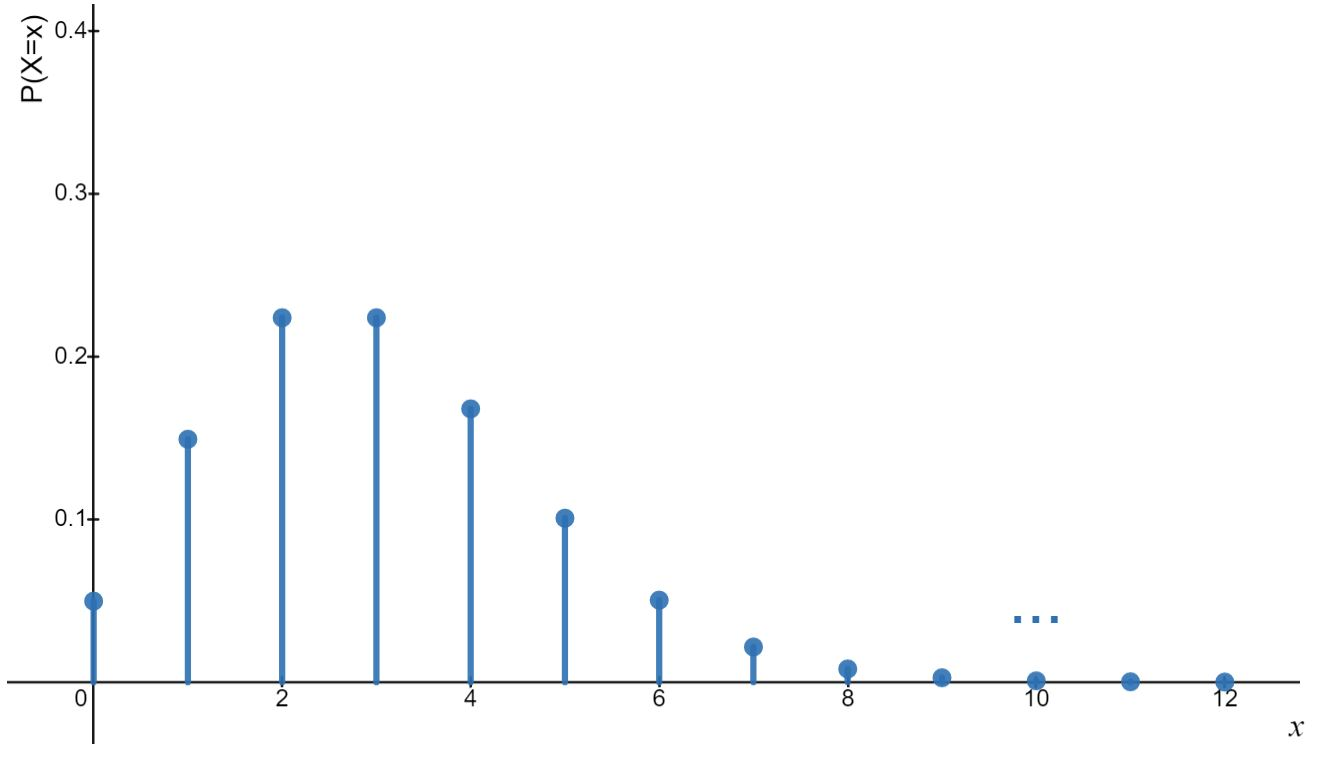
\includegraphics[width=0.75\linewidth]{./figures/poisson1} 

}

\caption{Probability mass function for Pois(3)}\label{fig:pois1}
\end{figure}

\begin{figure}

{\centering 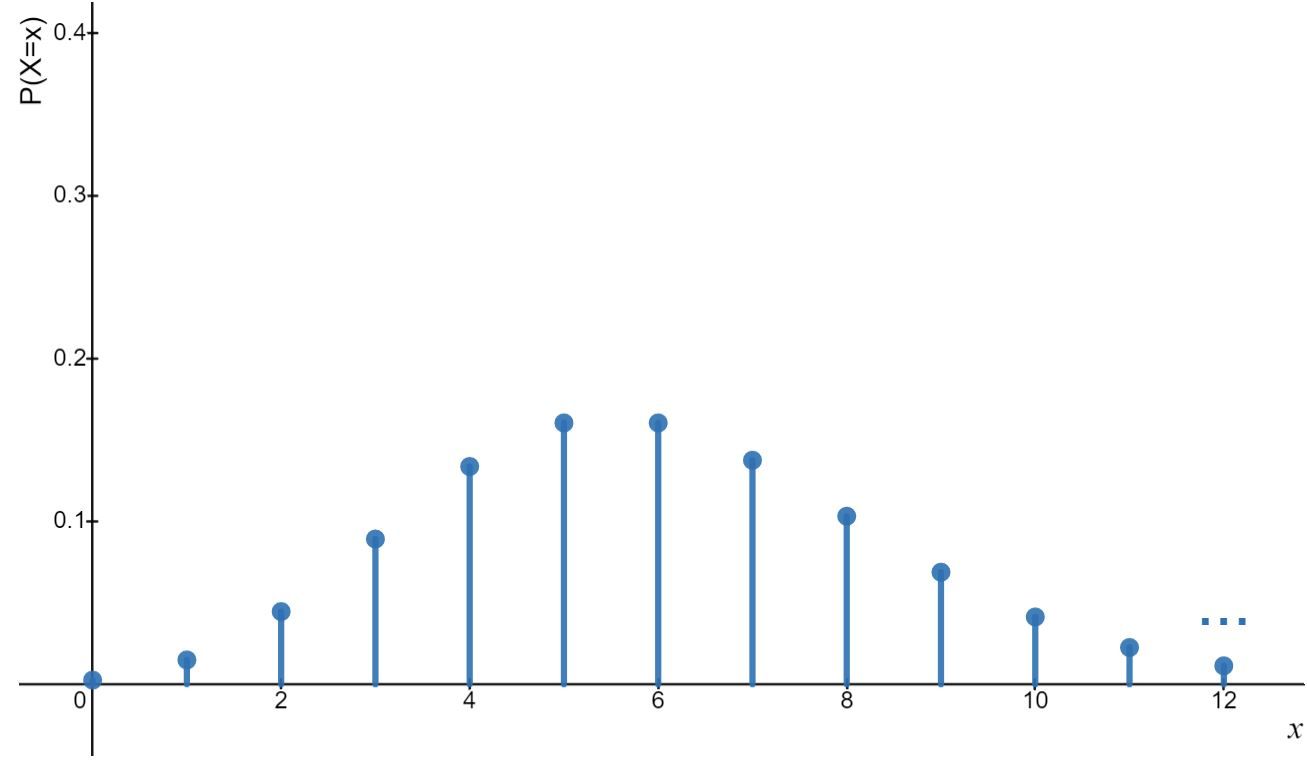
\includegraphics[width=0.75\linewidth]{./figures/poisson2} 

}

\caption{Probability mass function for Pois(6)}\label{fig:pois2}
\end{figure}

\begin{definition}
Given a random variable following a Poisson distribution \(X\sim \text{Pois}(\lambda)\) has mass function given by:

\[\text{P}(X=x) = \frac{\lambda^x e^{-\lambda}}{x!} \]
where \(x=0,1,2, \dots\), and \(\lambda>0\).
\end{definition}

Although the probabilities attached to higher values of \(x\) are positive, they quickly become very small. The mean rate \(\lambda\) does not need to be a whole number, even though the count in any given interval does need to be a whole number. As with the binomial distribution, tables are given of the CDF of the Poisson distribution.

\begin{example}

A company operates a helpdesk hotline service. Incoming calls to the hotline arrive at a mean rate of \(3.5\) per minute and outgoing calls are made at a rate of \(4.2\) per minute. Find the probability that

\begin{enumerate}
\def\labelenumi{\alph{enumi})}
\item
  at least five calls arrive in one minute.
\item
  exactly five calls arrive in one minute.
\item
  at most 7 calls are outgoing in one minute.
\item
  between \(4\) and \(9\) calls inclusive are outgoing in one minute.
\end{enumerate}

\emph{solution}

\begin{enumerate}
\def\labelenumi{\alph{enumi})}
\item
  \(\text{P}(X\geq 5) = 1 - \text{P}(X\leq 4) = 1-0.7254 = 0.2746\)
\item
  \(\text{P}(X=5) = \text{P}(X\leq 5) - \text{P}(X\leq 4) = 0.8576 - 0.7254 = 0.1322\)
\item
  \(\text{P}(Y\leq 7) = 0.9361\)
\item
  \(\text{P}(4\leq Y \leq 9 ) = \text{P}(Y\leq 9) - \text{P}(Y\leq 3) = 0.9889 - 0.3954 = 0.5935\).
\end{enumerate}

\end{example}

\hypertarget{further-properties}{%
\subsection{Further properties}\label{further-properties}}

An important aspect of the Poisson model is the uniform average rate. This means that we assume events occur at the same rate over the interval. If the size of the interval changes, then we must change the mean rate in direct proportion with that change of size.

\begin{example}[hotline continued]
Again assume calls to the hotline are incoming with rate \(3.5\) per minute. Find the probability that

\begin{enumerate}
\def\labelenumi{\alph{enumi})}
\item
  at least \(20\) calls arrive at the exchange in a \(4\) minute period.
\item
  at most \(1\) call arrives in a \(12\) second period.
\end{enumerate}

\emph{solution}

\begin{enumerate}
\def\labelenumi{\alph{enumi})}
\tightlist
\item
  If there are \(3.5\) calls per minute, then in a \(4\) minute period one expects a rate of \(3.5\times 4=14\) calls.
\end{enumerate}

Let \(W\) be the number of calls in a \(4\) minute period. Then \(W\sim\text{Pois}(14)\). Then,

\[\text{P}(W\geq 20) = 1- \text{P}(W\leq 19) = 1-0.9235 = 0.0765.\]

\begin{enumerate}
\def\labelenumi{\alph{enumi})}
\setcounter{enumi}{1}
\tightlist
\item
  As \(12\) seconds is one fifth of a minute, so we would expect a rate of \(3.5\div 5 = 0.7\) calls.
\end{enumerate}

Let \(Z\) be the number of calls in a \(12\) second period. Then,

\[\text{P}(Z\leq 1) = 0.8442\]
\end{example}

The second useful property is that different Poisson variables can be added together and yield another Poisson distribution whose rate parameter is the sum of the individual rates.

\begin{theorem}
That is, if \(X\sim \text{Pois}(\lambda)\) and \(Y\sim \text{Pois}(\mu)\) then
\[X+Y \sim \text{Pois}(\lambda+\mu)\]
\end{theorem}

\begin{proof}
Omitted for now. In your second year course you will learn moment generating functions which makes the proof very easy.
\end{proof}

\begin{example}
Suppose in a game of football the home team scores goals at a rate of \(2\) per match, and the away team scores goals at a rate of \(3\) per match. Then you would expect the total number of goals between these two teams to occur at a rate of \(5\) per match.

In this context for a particular pair of teams this may not be a realistic model. Why?
\end{example}

\hypertarget{mean-and-variance-1}{%
\section{Mean and Variance}\label{mean-and-variance-1}}

In this section we consider the mean and variance of the Poisson distribution.

We need a few Mathematical preliminaries from Calculus.

:::\{.proposition name = ``characterisations of Euler's number''\}
A) For any real number \(x \in \mathbb{R}\) we have

\[e^x = \sum_{k=0}^{\infty} \frac{x^k}{k!}\]
B)
\[ \lim_{n\to \infty} \left( 1+\frac{x}{n} \right)^n = e^x\]
:::

\begin{theorem}
Let \(X\) be a Poisson distributed random variable with rate \(\lambda\), that is \(X\sim \text{Pois}(\lambda)\). Then

\[\text{E}[X]  = \lambda\]
and
\[\text{Var}[X] = \lambda\]
\end{theorem}

\begin{proof}
\[\text{E}[X] = \sum_{x=0}^{\infty}x\frac{\lambda^x e^{-\lambda}}{x!}\]
\[ =\lambda e^{-\lambda} \sum_{x=1}^{\infty}\frac{\lambda^{(x-1)}}{(x-1)!} \]
\[=\lambda e^{-\lambda} \sum_{y=0}^{\infty}\frac{\lambda^{y}}{y!} \]
\[=\lambda e^{-\lambda} e^{\lambda}  \]
\[ = \lambda .\]
For the variance consider

\[\text{E}[X(X-1)] = \sum_{x=0}^{\infty}x(x-1)\frac{\lambda^x e^{-\lambda}}{x!}\]
\[ =\lambda^2e^{-\lambda} \sum_{x=2}^{\infty}\frac{\lambda^{x-2}}{(x-2)!}\]
\[ =\lambda^2e^{-\lambda} \sum_{y=0}^{\infty}\frac{\lambda^y}{y!}\]
\[ =\lambda^2e^{-\lambda} e^{\lambda}\]
\[ =\lambda^2\]
As \(\text{E}[X(X-1)] = \text{E}[X^2] - \text{E}[X^2]\), we can rearrange and find that

\[\text{E}[X^2] = \lambda^2 + \lambda \]

And as the variance \(\text{Var}[X] = \text{E}[X^2] - \text{E}[X]^2\), we have:

\[\text{Var}[X] = \lambda^2 + \lambda - \lambda ^2 = \lambda .\]
\end{proof}

\hypertarget{deriving-the-poisson-mass-function}{%
\section{Deriving the Poisson mass function}\label{deriving-the-poisson-mass-function}}

The Poisson distribution is intimately linked to the binomial distribution. The aim of this section is to show you why the mass function has the form given in the definition.

Suppose events occur as a result of a Poisson process independently and at a uniform rate \(\lambda\) in a given time interval. Divide up the time period into a large number of smaller intervals, \(n\) say, such that the chance of two events happening in one interval in negligible. The probability of an event happening in one of the small intervals is \(\lambda / n\).

Letting \(X\) be the random variable representing the number of small intervals that contain an event, then we can see that this is on the one hand binomially distributed for fixed \(n\). We have

\[ \text{P}(X=x) = {}^nC_{x} \left(\frac{\lambda}{n}\right)^x \left( 1- \frac{\lambda}{n}\right)^{n-x}\]

\[ = \lambda^{x} \underbrace{\frac{^nC_{x}}{n^x}}_{1} \underbrace{\left( 1- \frac{\lambda}{n}\right)^{n}}_{2}\underbrace{\left( 1- \frac{\lambda}{n}\right)^{-x}}_{3} \]

We consider what happens when we increase \(n\), and consider each term separately (which we are allowed to do for convergent sequences).

For term \(2\), as \(n\) gets larger the number inside the bracket gets close to \(1\), and so overall the limit is \(1\).

For term \(3\) this can be seen to be equal to \(e^{-\lambda}\) by the proposition (B).

The first term \(1\), can be manipulated as follows:

\[\lim_{n\to \infty}\frac{^nC_{x}}{n^x} = \lim_{n\to \infty} \frac{n!}{(n-x)!x!n^x}\]

\[ =\frac{1}{x!}  \lim_{n\to \infty} \frac{n(n-1)(n-2)\dots(n-x+1)}{n^x}\]

\[ =\frac{1}{x!}  \lim_{n\to \infty} \frac{n}{n}\frac{(n-1)}{n}\frac{(n-2)}{n}\dots \frac{(n-x+1)}{n}\]
\[ =\frac{1}{x!}  \lim_{n\to \infty} \frac{n}{n}\frac{(n-1)}{n}\frac{(n-2)}{n}\dots \frac{(n-x+1)}{n}\]
\[ =\frac{1}{x!}  \lim_{n\to \infty} \frac{(n-1)}{n}\frac{(n-2)}{n}\dots \frac{(n-x+1)}{n}\]
\[ =\frac{1}{x!}  \lim_{n\to \infty} \left(1 - \frac{1}{n}\right)\lim_{n\to \infty}\left(1 - \frac{2}{n}\right)\dots \lim_{n\to \infty} \left(1 - \frac{x-1}{n}\right)\]
And all of these limits are \(1\).

Altogether then,

\[lim_{n\to \infty} {}^nC_{x} \left(\frac{\lambda}{n}\right)^x \left( 1- \frac{\lambda}{n}\right)^{n-x}  = \lambda^x \times \frac{1}{x!} \times e^{-\lambda}\times 1 = \frac{\lambda^xe^{-\lambda}}{x!}.\]
This is the probability of observing \(x\) events in the whole time interval.

The other side of this relationship is that a Poisson distribution can be used to approximate the binomial distribution.

\begin{theorem}
If \(\pi\) is small and \(n\) is large then, a binomial distribution can be approximated by a Poisson distribution with rate parameter equal to the mean of the binomial distribution.

\[\text{Binom}(n,\pi) \approx \text{Pois} (\lambda)\]
Where we set \(\lambda = n\pi.\)

\emph{proof}
Omitted.
\end{theorem}

\hypertarget{exercises-week-4}{%
\section{Exercises week 4}\label{exercises-week-4}}

\begin{exercise}
Ropes are tested at a certain breaking strain. According to past experience a quarter of all ropes break at this strain. If \(4\) identical ropes are tested, write down the probability distribution of the number of ropes breaking.
\end{exercise}

\begin{exercise}

If it estimated that \(20\%\) of all individuals carry anibodies to a particular virus. What is the probability that in a group of \(20\) randomly selected individuals:

\begin{enumerate}
\def\labelenumi{\alph{enumi})}
\item
  More than \(8\) have antibodies.
\item
  Exactly \(6\) have antibodies.
\item
  Fewer than \(4\) have antibodies.
\item
  Between \(3\) and \(6\) inclusive have antibodies.
\end{enumerate}

\end{exercise}

\begin{exercise}

A car salesperson knows from past experience that she will make a sale to \(30\%\) of her customers. Find the probability that in \(20\) randomly selected sales pitches she makes a sale to

\begin{enumerate}
\def\labelenumi{\alph{enumi})}
\item
  More than 4 customers
\item
  Fewer than \(7\) customers
\item
  Exactly \(6\) customers
\item
  between \(4\) and \(10\) exclusive.
\end{enumerate}

\end{exercise}

\begin{exercise}
A footballer takes a free kick and scores a goal on \(10\%\) of occasions. Find the probability that in a match in which \(10\) free kicks are taken

\begin{enumerate}
\def\labelenumi{\alph{enumi})}
\item
  She scores at least two goals
\item
  She scores exactly two goals
\item
  She scores \(3\) goals or fewer.
\end{enumerate}

These are goals from free kicks alone. What assumptions do you need to make, and to what extent do you think these are reasonable?
\end{exercise}

\begin{exercise}
A statistics lecturer sets a test involving \(20\) multiple choice questions. They want to choose a pass mark so that the chance of passing a student who guesses every question is less than \(5/%
\). What should the pass mark be?
\end{exercise}

\begin{exercise}
The game of \emph{advanced Chuck-a-luck} is an extension of the simple game from last week's exercises. The banker rolls \(n\) dice and the player wins £\(x\) if the number that the player guesses appears on \(x\) of the \(n\) dice. As before he loses his £\(1\) stake if the number does not come up on any of the dice.

\begin{enumerate}
\def\labelenumi{\alph{enumi})}
\item
  Write down the probability mass function of \(X\).
\item
  Show that \(\text{E}[X] = \frac{n}{6} - \left(\frac{5}{6}\right)^n\)
\end{enumerate}

(Hint you might want to build up to part (a) in particular by picking values of \(n=1,2,3,\dots\) and pattern spotting.)
\end{exercise}

\begin{exercise}

A biologist on a field trip is studying biodiversity and has found that the number of plant species in a \(1 \  \text{m}^2\) quadrat follows a Poisson distribution with mean \(6\).

\begin{enumerate}
\def\labelenumi{\alph{enumi})}
\tightlist
\item
  Find the probability that the number of plant species in any given \(1 \  \text{m}^2\) quadrat is;
\end{enumerate}

\begin{enumerate}
\def\labelenumi{(\roman{enumi})}
\item
  at least 8
\item
  less than or equal to \(8\)
\item
  exactly \(8\)
\item
  between \(6\) and \(12\) inclusive
\end{enumerate}

\begin{enumerate}
\def\labelenumi{\alph{enumi})}
\setcounter{enumi}{1}
\tightlist
\item
  Find the probability that in a quadrat of area \(0.5 \  \text{m}^2\), the number of plant species is
\end{enumerate}

\begin{enumerate}
\def\labelenumi{(\roman{enumi})}
\item
  at least \(3\)
\item
  fewer than \(5\)
\item
  exactly \(4\)
\item
  between \(3\) and \(6\) inclusive
\end{enumerate}

\end{exercise}

\begin{exercise}

When a car leaves a roduction line it is carefully examined for any signs of imperfection in the paintwork. Previous experience has shown the number of blemishes per car follows a Poisson distribution with mean \(0.4\).
a) Find the probability that a car has

\begin{enumerate}
\def\labelenumi{(\roman{enumi})}
\item
  at least one blemish
\item
  more than one blemish
\item
  exactly one blemish
\item
  no blemishes
\end{enumerate}

\begin{enumerate}
\def\labelenumi{\alph{enumi})}
\setcounter{enumi}{1}
\tightlist
\item
  In \(1\) hour an inspector can examine \(20\) cars. Assuming that blemishes occur independently, find the probability that the inspector finds
\end{enumerate}

\begin{enumerate}
\def\labelenumi{(\roman{enumi})}
\item
  fewer than \(5\) blemishes
\item
  exactly five blemishes
\item
  at least one blemish
\end{enumerate}

\end{exercise}

\begin{exercise}

A traffic survey found that buses pass a checkpoint at an average rate of \(4.5\) per hour. Lorries pass the same checkpoint at the rate \(5\) per hour and coaches at the rate of \(1.5\) per hour.

\begin{enumerate}
\def\labelenumi{\alph{enumi})}
\tightlist
\item
  Find the probability that in \(1\) hour
\end{enumerate}

\begin{enumerate}
\def\labelenumi{(\roman{enumi})}
\item
  \(5\) or more buses pass the checkpoint
\item
  between \(10\) and \(15\) lorries inclusive pass the checkpoint
\item
  fewer than \(3\) buses pass the checkpoint
\end{enumerate}

\begin{enumerate}
\def\labelenumi{\alph{enumi})}
\setcounter{enumi}{1}
\item
  \begin{enumerate}
  \def\labelenumii{(\roman{enumii})}
  \tightlist
  \item
    At least \(8\) buses or coaches pass the checkpoint in an hour
  \end{enumerate}
\end{enumerate}

\begin{enumerate}
\def\labelenumi{(\roman{enumi})}
\setcounter{enumi}{1}
\item
  exactly \(15\) buses or coaches will pass the checkpoint in an hour
\item
  ten or fewer buses, lorries or coaches will pass the checkpoint in half an hour.
\end{enumerate}

\end{exercise}

\begin{exercise}

The numbers of emissions per minute from two radioactive rocks \(A\) and \(B\) are independent Poisson variables with means \(0.65\) and \(0.45\) respectively. Find the probability that

\begin{enumerate}
\def\labelenumi{(\alph{enumi})}
\item
  In a period of three minutes there are at least three emissions from \(A\).
\item
  In a period of two minutes there is a total of less than four emissions from \(A\) and \(B\) combined.
\end{enumerate}

\end{exercise}

\begin{exercise}

In a particular form of cancer, deformed blood corpuscles occur at random at the rate of \(10\) per \(1000\) corpuscles.

\begin{enumerate}
\def\labelenumi{\alph{enumi})}
\item
  Use an appropriate approximation to determine the probability that a random sample of \(200\) corpuscles taken from a cancerous area will contain no deformed corpuscles.
\item
  How large a sample should be taken in order to be \(99\%\) certain of there being at least one deformed corpuscle in the sample?
\end{enumerate}

\end{exercise}

\begin{exercise}[counting practice]

A box contains \(12\) golf balls, \(3\) of which are substandard. A random sample of \(4\) balls is selected, without replacement, from the box. The random variable \(R\) denotes the number of balls in the sample that are substandard.

\begin{enumerate}
\def\labelenumi{\alph{enumi})}
\item
\end{enumerate}

\begin{enumerate}
\def\labelenumi{(\roman{enumi})}
\tightlist
\item
  Show that the probability mass function of \(R\) satisfies
\end{enumerate}

\[\text{P}(R=r) = \frac{{}^3C_r \times {}^9C_{4-r}}{^{12}C_{4}} \]
(ii) Determine the probability that \(R=0\)

\begin{enumerate}
\def\labelenumi{(\roman{enumi})}
\setcounter{enumi}{2}
\tightlist
\item
  Determine the probability that there are fewer than two substandard balls.
\end{enumerate}

\begin{enumerate}
\def\labelenumi{\alph{enumi})}
\setcounter{enumi}{1}
\tightlist
\item
  A large bin contains \(5000\) used golf balls, \(1500\) of which are defective. The random variable \(X\) denotes the number of defective balls in a random sample of 20balls selected, without replacement,from the bin. Explain why \(X\) may be approximated as a binomial variable with parameters \(20\) and \(0.3\). Using the binomial model, calculate the probability that this sample contains
\end{enumerate}

\begin{enumerate}
\def\labelenumi{(\roman{enumi})}
\item
  fewer than \(5\) defective balls
\item
  at least \(7\) defective balls
\end{enumerate}

\begin{enumerate}
\def\labelenumi{\alph{enumi})}
\setcounter{enumi}{2}
\tightlist
\item
  The random variable \(Y\) denotes the number of defective golf balls in a sample of \(2000\), selected from a batch of \(200,000\) and of which \(3250\) are defective. Completely specify an approximate distribution for \(Y\) other than a binomial model.
\end{enumerate}

\end{exercise}

\begin{exercise}
The independent random variables \(X\) and \(Y\)have means \(2.5\) and \(1.5\) respectively. Obtain the mean and variance of the random variables below, and hence give a reason why they are not Poisson.
a) \(X-Y\)
b) \(2X+5\)
\end{exercise}

  \bibliography{book.bib,packages.bib}

\end{document}
